\chapter{Results interpretation}

Based on the results of the different experiments I made, I will try to answer in this chapter to three main questions:
\begin{enumerate}
  \item Compared to other available solutions, how good is the current configuration chosen by INGInious to face the responsiveness challenge of the platform?  How much better could it be?  How easy would it be to improve it?
  \item Could there be a solution tailor-made for the specific case of INGInious?  What would it be?  What would it take to use it?
  \item What would be the cost of providing a stronger/safer isolation to the containers used by INGInious?  What opportunities could it bring?
\end{enumerate}

\section{Current INGInious situation}
We will here consider the first question:
\begin{center}
  \say{\textit{Compared to other available solutions, how good is the current configuration chosen by INGInious to face the responsiveness challenge of the platform?  How much better could it be?  How easy would it be to improve it?}}
\end{center}

The current configuration of INGInious is the following:
\begin{center}
\begin{tabular}{rl}
  \textbf{Container manager} & Docker \\
  \textbf{Base image} & Centos \\
  \textbf{Storage driver} & overlay2 \\
  \textbf{Container runtime} & runc \\
  \textbf{Control group version} & v1 \\
  \textbf{Rootless containers} & no \\
\end{tabular}
\end{center}

This configuration is quite decent, and gives good performances, their is mainly one change that can improve those.  But let's analyse this step by step.

\subsubsection{Storage driver}
Overlay2 (referenced later as simply overlay) is the storage driver that Docker recommands to use by default (when OverlayFS is supported on the host).  Its layer mechanism allows to limit the redundancy of information when you use the same base image to create different images.  And its file-based copy-on-write strategy gives overal good performances.

\begin{figure}[h!]
  \begin{center}
    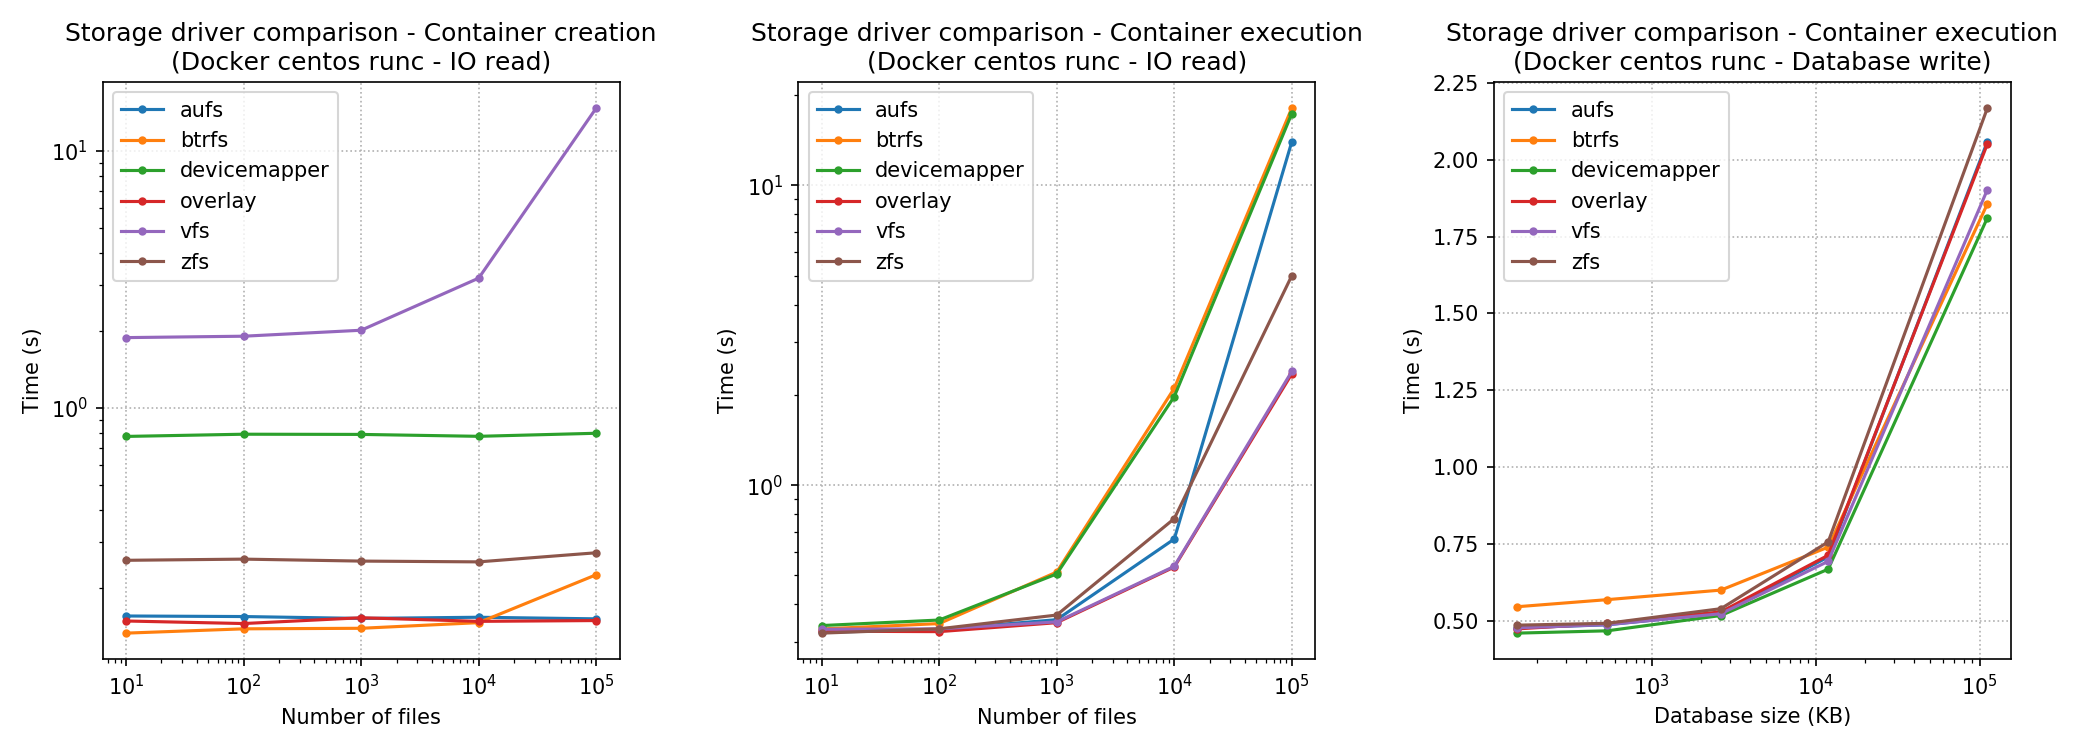
\includegraphics[width=\linewidth]{images/question-1-storage-driver-Docker-centos-runc---Database-write.png}
    \caption{Storage driver performance comparison for Centos container, launched with Docker and runc}
    \label{fig:q1:storage-driver}
  \end{center}
\end{figure}

On Figure \ref{fig:q1:storage-driver}, we can see how much it cost to have a full-copy mechanism like vfs for each container creation.  We can also see that overlay, aufs and btrfs offers similar performances for the creation.  The main differences between those three is shown by their performance when solicitating I/O.  
\begin{itemize}
  \item Aufs, even though performing similarly to overlay in all the other cases (not shown here) and relying on the same union file system mechanism as overlay, gets far behind the latest when a lot of read operations are done.  This most likely comes from one big difference in the implementation of those two union file system: when a file is opened with OverlayFS, all the operations on it are directly managed by the underlying file systems.  This simplify the implementation, and improve the performances quite a lot as we can see on the second graph of the figure.  (For this test, for each \texttt{openat} system call, four \texttt{read} system call are done)
  \item On the last graph of the figure (on the right), we can see the advantage of using block-based copy-on-write, when modifying big files.  Indeed, when doing so, where overlay and aufs will need to copy the whole file before modifying it, the other solutions will only need to copy the file system blocks needing to be modified (or not even copy the file in the case of vfs).  We can see that devicemapper handles this a little bit better than btrfs, but given the much higher container creation cost of the first one, it will most likely be more intersting to use btrfs in most cases.
\end{itemize}
One more reason to justify the use of overlay is that in most container use cases, read operations are the most important ones.  Normally, no large amount of data should be written in the container file systems, volumes (external storage from the host, mounted into the container file system) should specifically be used for that purpose as it provide nearly native writing performances and the data persists, even after the end of the container life cycle.

\subsubsection{Base image}

\subsubsection{Container runtime}

\subsubsection{Container manager}

\subsubsection{Final configuration}

\begin{center}
\begin{tabular}{rl}
  \textbf{Container manager} & Docker \\
  \textbf{Base image} & Alpine/Centos \\
  \textbf{Storage driver} & overlay2 \\
  \textbf{Container runtime} & crun \\
  \textbf{Control group version} & v1 \\
  \textbf{Rootless containers} & no \\
\end{tabular}
\end{center}

As we can see, the final configuration is not that much different from the original one.  The quick answer to the original questions would be:
\paragraph{}\textit{Compared to other available solutions, how good is the current configuration chosen by INGInious to face the responsiveness challenge of the platform?}  The current configuration is good.  It could be improved, but is definitely not the worse one.  The choice of going with Docker was the most soundfull when INGInious was created, and it is still the case now.  The current storage driver offers great performances for almost every cases, only some specific case, sollicitating a lot of IO operations on big files, can give an advantage to another storage driver, btrfs.  The choice of a Centos base image is not bad either, but the size of the image being greater than Alpine's one, except for the situations where Centos offered better write performances, using Alpine seems to be better.  The move here might then be to go for an hybrid solution, using Centos only in situations where its small writing performance advantage become meaningfull.  
\paragraph{}\textit{How much better could it be?}  As we have seen, changing the current container runtime makes a significant difference.  The c implementation of \texttt{crun} is claimed to be twice as fast as the go implementation of \texttt{runc} by \texttt{crun}'s contributors.  And we can definitely see the difference.  The change of base Image though doesn't show as obvious improvement.
\paragraph{}\textit{How easy would it be to improve it?}  This is the real good news, it truely is super easy to apply the most significant change.  You only need to install \texttt{crun}, reconfigure Docker to use it by default, and you are good to go, no change as to be done to INGInious!  For the base of the base image the story is different though, as it would require to change all the containers images, which is a lot of work.

\section{Variabilities influence}

\clearpage
\subsubsection{Kata-container's case}
Those same storage drivers (same implementation) behave very differently when using virtualization-based containers, with Kata-container.  The common configuration will now be:

\begin{tabular}{rl}
   \textbf{Container manager} & Docker \\
   \textbf{Container runtime} & kata-runtime \\
   \textbf{Base image} & Alpine \\
   \textbf{Control group} & v1 \\
   \textbf{Rootless} & No 
\end{tabular}

The behaviour of Kata-container using qemu with devicemapper storage driver correspond to the behaviour of this same driver but with Kata-container using Firecracker as hypervisor.

\begin{figure}[h!]
    \begin{subfigure}{.5\textwidth}
      \centering
      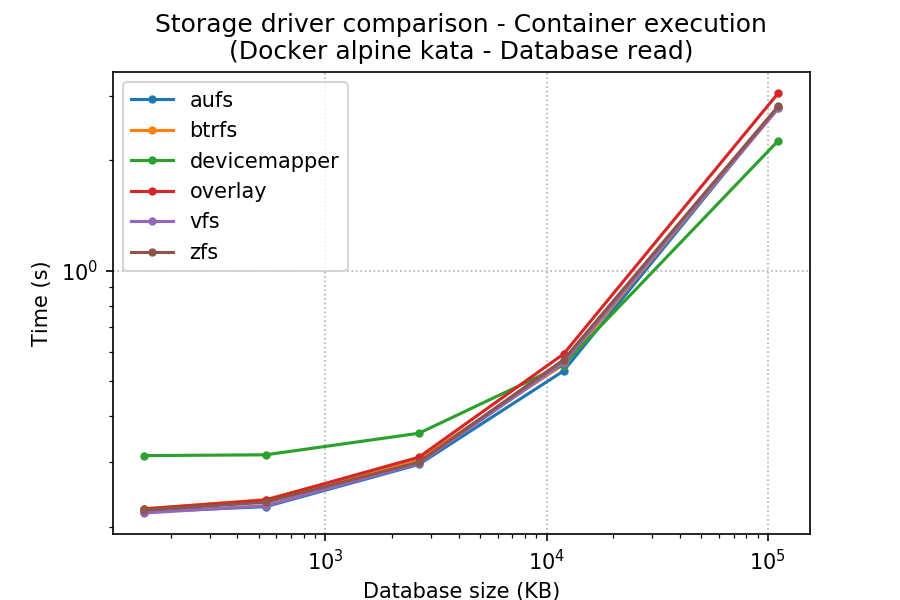
\includegraphics[width=\linewidth]{images/storage-driver/storage-driver-execution-Docker-alpine-kata---Database-read.png}
      \caption{Execution time of containers used for database reading performance test.}
      \label{fig:storage-driver:kata:db-read-exec}
    \end{subfigure}
    \begin{subfigure}{.5\textwidth}
      \centering
      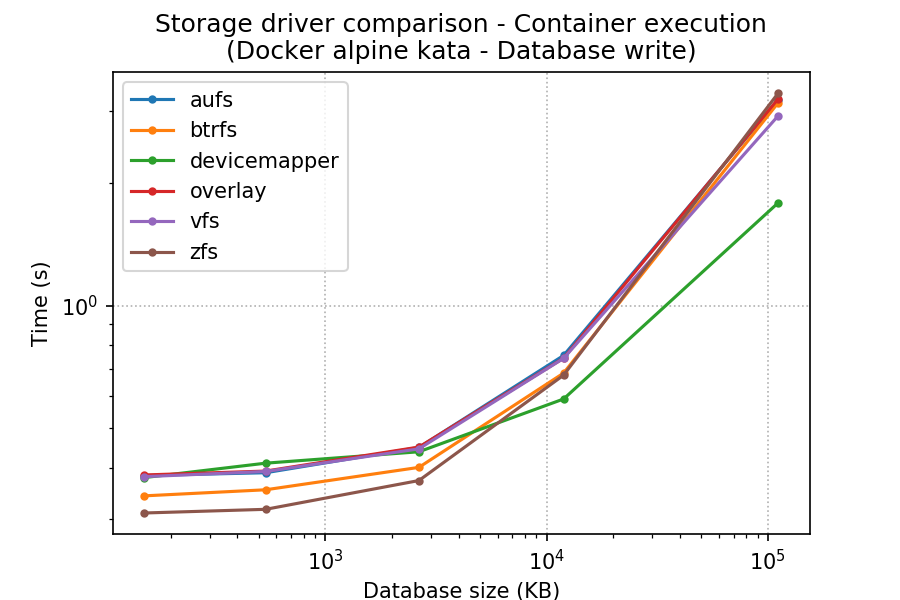
\includegraphics[width=\linewidth]{images/storage-driver/storage-driver-execution-Docker-alpine-kata---Database-write.png}
      \caption{Execution time of containers used for database reading performance test.}
      \label{fig:storage-driver:kata:db-write-exec}
    \end{subfigure}
    
    \begin{subfigure}{.5\textwidth}
      \centering
      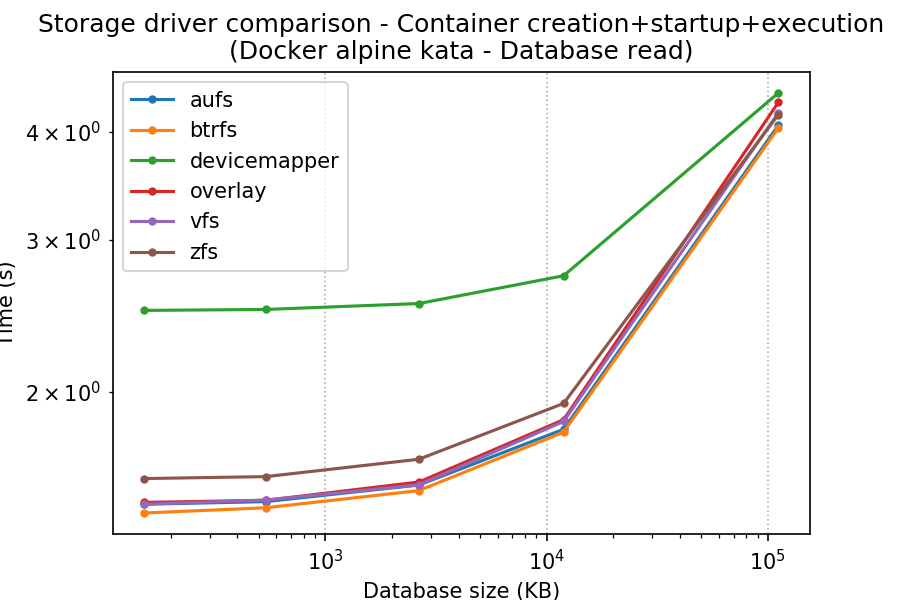
\includegraphics[width=\linewidth]{images/storage-driver/storage-driver-full-Docker-alpine-kata---Database-read.png}
      \caption{Creation, startup and execution time of containers used for database reading performance test.}
      \label{fig:storage-driver:kata:db-read-full}
    \end{subfigure}
    \begin{subfigure}{.5\textwidth}
      \centering
      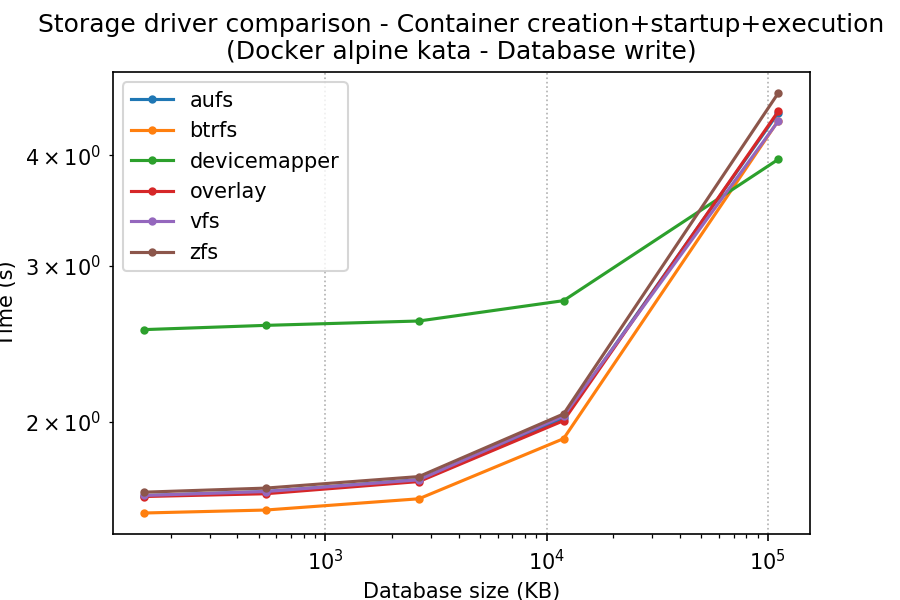
\includegraphics[width=\linewidth]{images/storage-driver/storage-driver-full-Docker-alpine-kata---Database-write.png}
      \caption{Creation, startup and execution time of containers used for database writing performance test.}
      \label{fig:storage-driver:kata:db-write-full}
    \end{subfigure}
    
    \caption{Database read and write tests for containers launched with Docker and Kata-Container (qemu), based on an Alpine image}
    \label{fig:storage-driver:kata:db}
\end{figure}

\begin{figure}[!h]
    
    \begin{subfigure}{.5\textwidth}
      \centering
      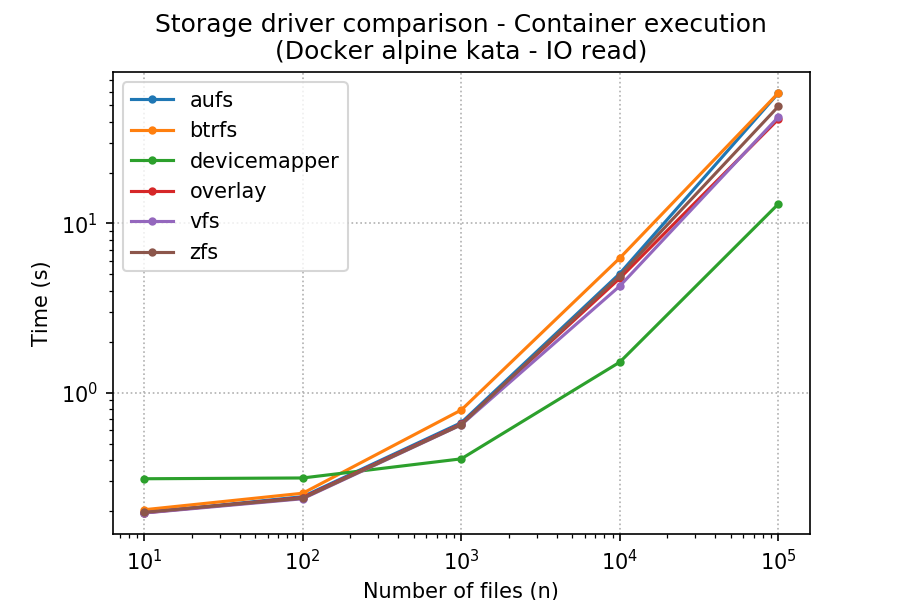
\includegraphics[width=\linewidth]{images/storage-driver/storage-driver-execution-Docker-alpine-kata---IO-read.png}
      \caption{Average total reading time for n files.}
      \label{fig:storage-driver:kata:io-read-exec}
    \end{subfigure}
    \begin{subfigure}{.5\textwidth}
      \centering
      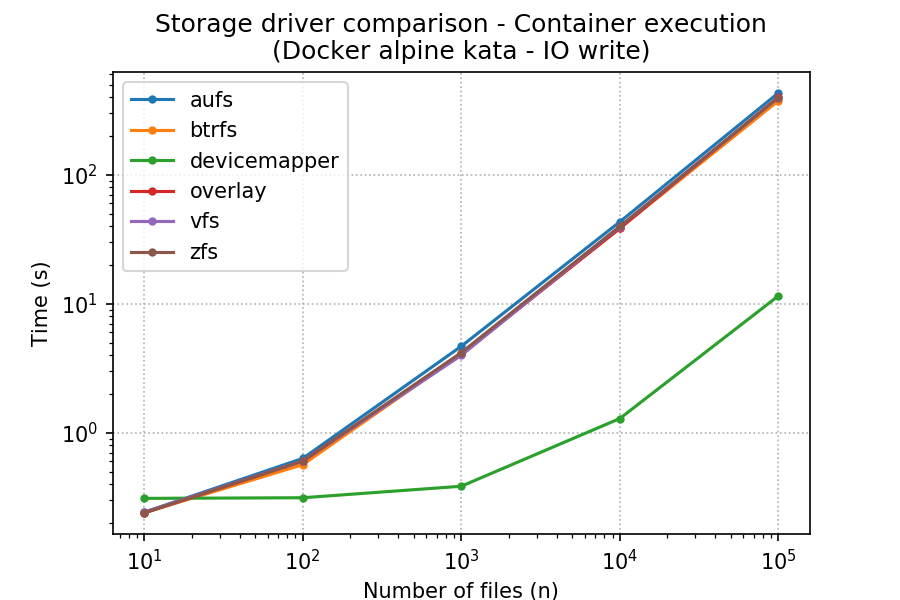
\includegraphics[width=\linewidth]{images/storage-driver/storage-driver-execution-Docker-alpine-kata---IO-write.png}
      \caption{Average extracting time of n files from one (non-compressed) archive.}
      \label{fig:storage-driver:kata:io-write-exec}
    \end{subfigure}
    
    \begin{subfigure}{.5\textwidth}
      \centering
      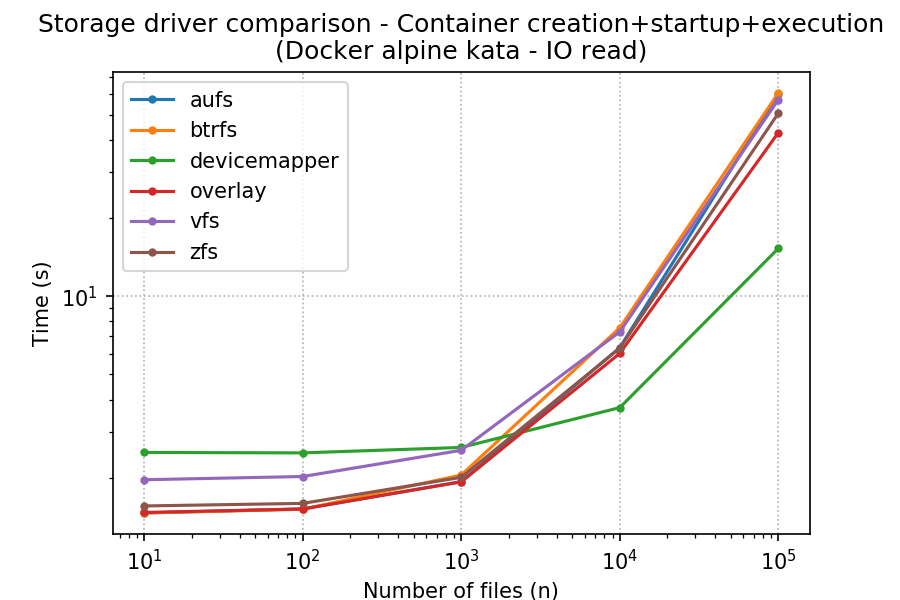
\includegraphics[width=\linewidth]{images/storage-driver/storage-driver-full-Docker-alpine-kata---IO-read.png}
      \caption{Average creation, startup and execution time of containers used for IO reading performance test.}
      \label{fig:storage-driver:kata:io-read-full}
    \end{subfigure}
    \begin{subfigure}{.5\textwidth}
      \centering
      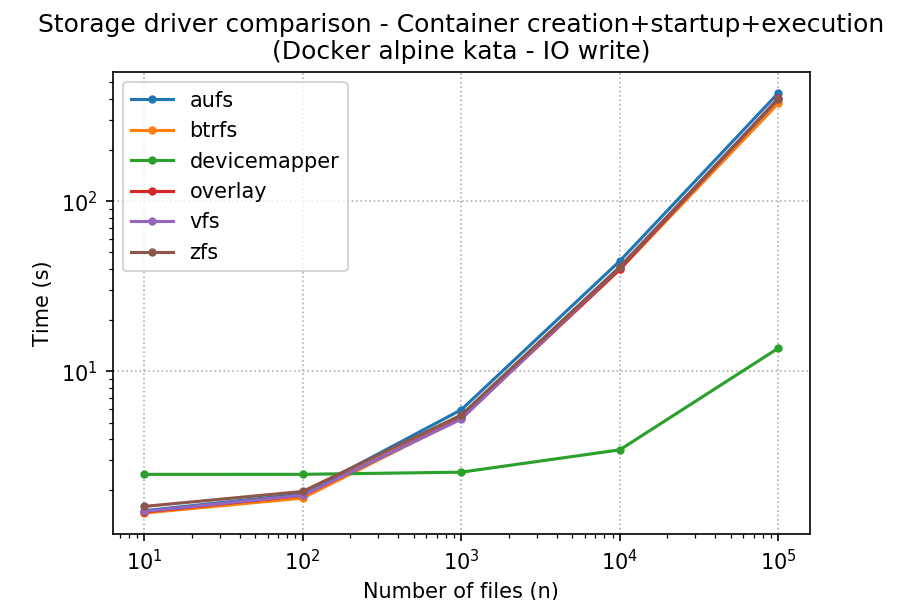
\includegraphics[width=\linewidth]{images/storage-driver/storage-driver-full-Docker-alpine-kata---IO-write.png}
      \caption{Average creation, startup and execution time of containers used for IO reading performance test.}
      \label{fig:storage-driver:kata:io-write-full}
    \end{subfigure}
    
    \caption{IO read and write tests for containers launched with Docker and Kata-Container (qemu), based on an Alpine image}
\end{figure}

\paragraph{}The creation of containers doesn't change that much with kata-container, neither does the startup, everything is just a little bit slower.  For the execution though, thinks get interesting.  Passed a certain point, devicemapper appear to be the only viable solution, and that turning point arrives quite quickly.  As you can see on Figure \ref{fig:storage-driver:kata:io-read-exec} and Figure \ref{fig:storage-driver:kata:io-write-exec}, all other storage drivers follow about the same curve.  It seems that the virtual block devices of devicemapper go well with virtualized solutions.  It kind of makes sense, but unfortunetly I can not explain it.  We can observe this same thing with the database tests (Figure \ref{fig:storage-driver:kata:db}), but it is less obvious than with the other ones.

\clearpage
\subsubsection{LXD's case}
Here the implementation of the storage drivers is different, and less of them are available.  The common configuration will be:

\begin{tabular}{rl}
   \textbf{Container manager} & LXD \\
   \textbf{Container runtime} & LXC \\
   \textbf{Base image} & Alpine \\
   \textbf{Control group} & v1 \\
   \textbf{Rootless} & No 
\end{tabular}

\begin{figure}[h!]
    \begin{subfigure}{.5\textwidth}
      \centering
      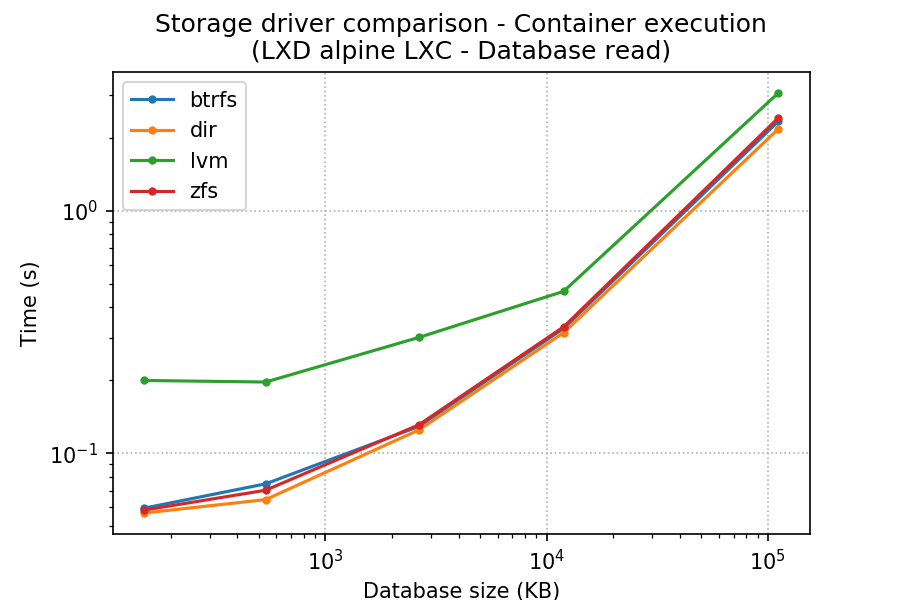
\includegraphics[width=\linewidth]{images/storage-driver/storage-driver-execution-LXD-alpine-LXC---Database-read.png}
      \caption{Execution time of containers used for database reading performance test.}
      \label{fig:storage-driver:lxc:db-read-exec}
    \end{subfigure}
    \begin{subfigure}{.5\textwidth}
      \centering
      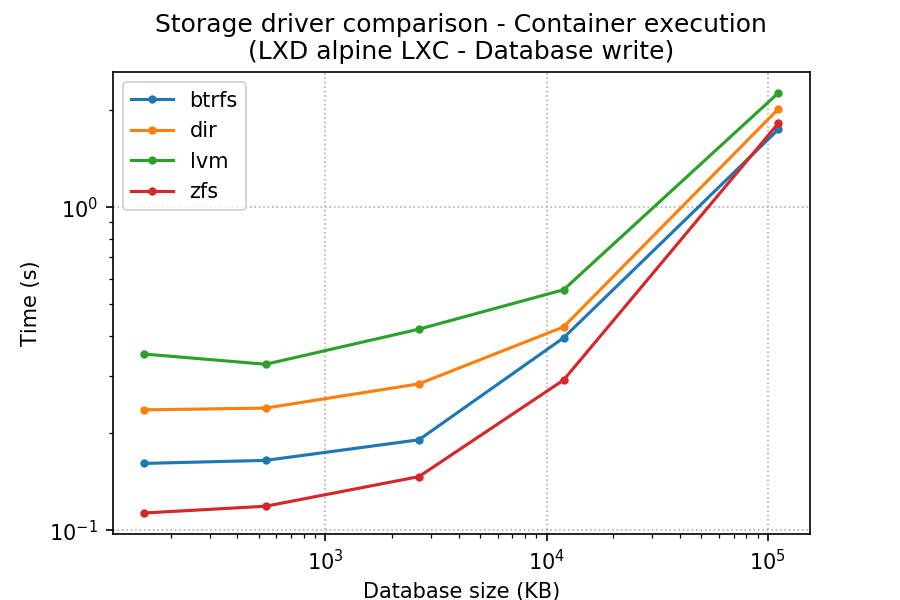
\includegraphics[width=\linewidth]{images/storage-driver/storage-driver-execution-LXD-alpine-LXC---Database-write.png}
      \caption{Execution time of containers used for database reading performance test.}
      \label{fig:storage-driver:lxc:db-write-exec}
    \end{subfigure}
    
    \begin{subfigure}{.5\textwidth}
      \centering
      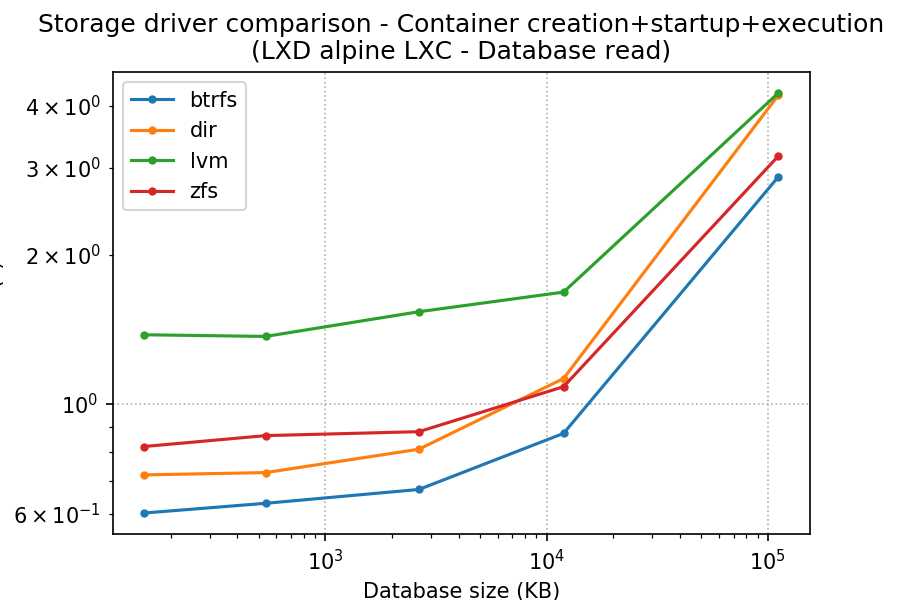
\includegraphics[width=\linewidth]{images/storage-driver/storage-driver-full-LXD-alpine-LXC---Database-read.png}
      \caption{Creation, startup and execution time of containers used for database reading performance test.}
      \label{fig:storage-driver:lxc:db-read-full}
    \end{subfigure}
    \begin{subfigure}{.5\textwidth}
      \centering
      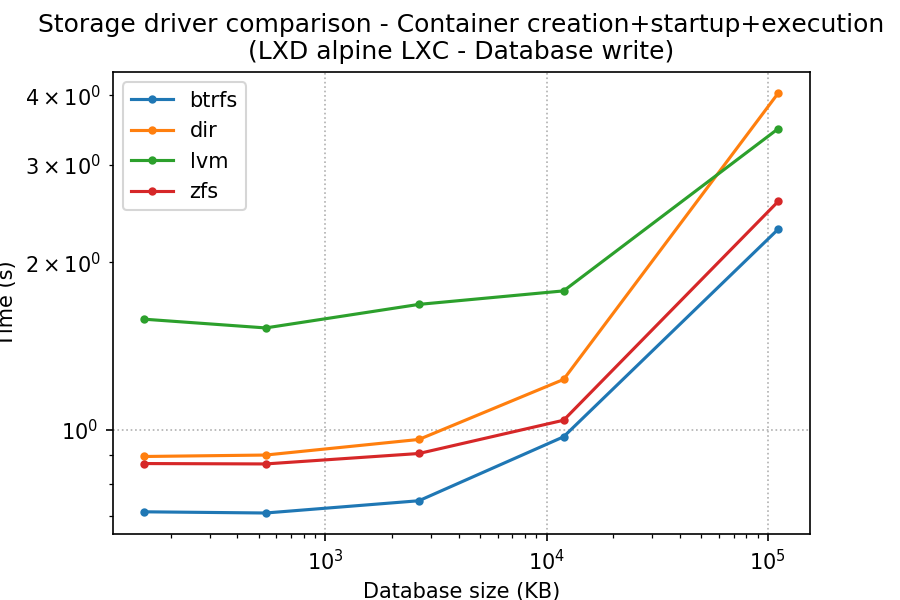
\includegraphics[width=\linewidth]{images/storage-driver/storage-driver-full-LXD-alpine-LXC---Database-write.png}
      \caption{Creation, startup and execution time of containers used for database writing performance test.}
      \label{fig:storage-driver:lxc:db-write-full}
    \end{subfigure}
    
    \caption{Database read and write tests for containers launched with LXD and LXC, based on an Alpine image}
    \label{fig:storage-driver:lxc:db}
\end{figure}

\begin{figure}[!h]
    \begin{subfigure}{.5\textwidth}
      \centering
      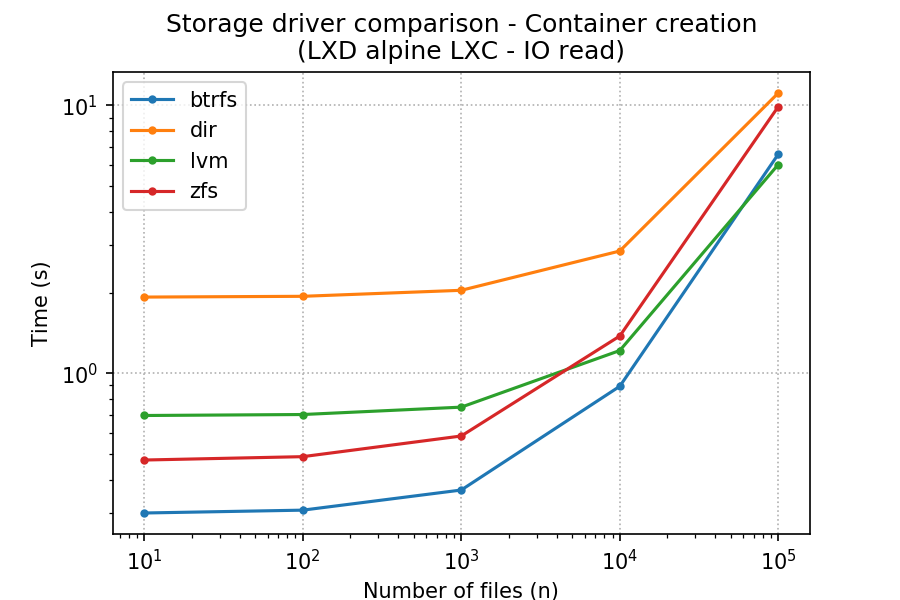
\includegraphics[width=\linewidth]{images/storage-driver/storage-driver-creation-LXD-alpine-LXC---IO-read.png}
      \caption{Average creation time of containers depending on the number of files in one folder.}
      \label{fig:storage-driver:lxc:io-read-create}
    \end{subfigure}
    \begin{subfigure}{.5\textwidth}
      \centering
      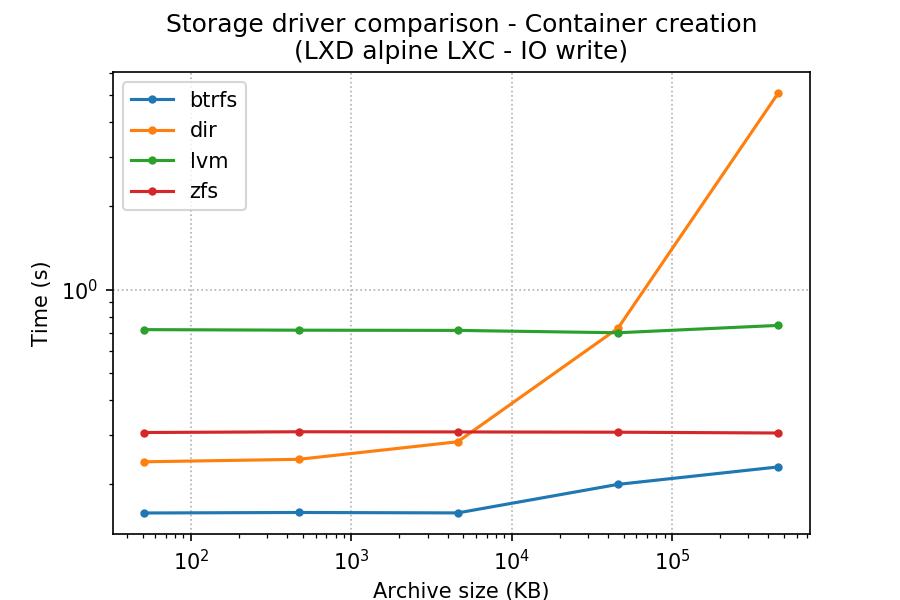
\includegraphics[width=\linewidth]{images/storage-driver/storage-driver-creation-LXD-alpine-LXC---IO-write.png}
      \caption{Average creation time of containers depending on the size of the archive containing all the files.}
      \label{fig:storage-driver:lxc:io-write-create}
    \end{subfigure}
    
    % \begin{subfigure}{.5\textwidth}
    %   \centering
    %   \includegraphics[width=\linewidth]{images/storage-driver/storage-driver-startup-LXD-alpine-LXC---IO-read.png}
    %   \caption{Starting time of containers used for IO reading performance test.}
    %   \label{fig:storage-driver:lxc:io-read-start}
    % \end{subfigure}
    % \begin{subfigure}{.5\textwidth}
    %   \centering
    %   \includegraphics[width=\linewidth]{images/storage-driver/storage-driver-startup-LXD-alpine-LXC---IO-write.png}
    %   \caption{Starting time of containers used for IO writing performance test.}
    %   \label{fig:storage-driver:lxc:io-write-start}
    % \end{subfigure}
    
    \begin{subfigure}{.5\textwidth}
      \centering
      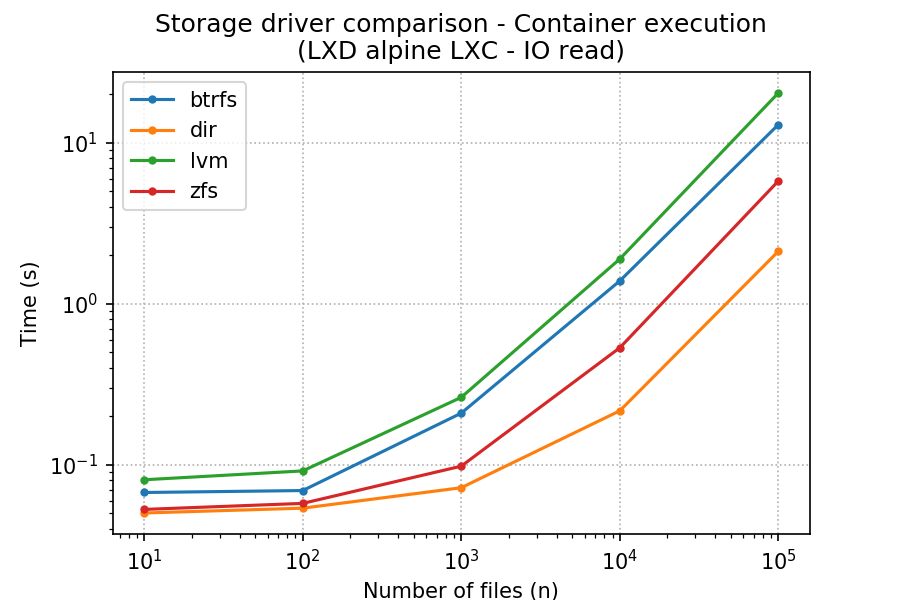
\includegraphics[width=\linewidth]{images/storage-driver/storage-driver-execution-LXD-alpine-LXC---IO-read.png}
      \caption{Average total reading time for n files.}
      \label{fig:storage-driver:lxc:io-read-exec}
    \end{subfigure}
    \begin{subfigure}{.5\textwidth}
      \centering
      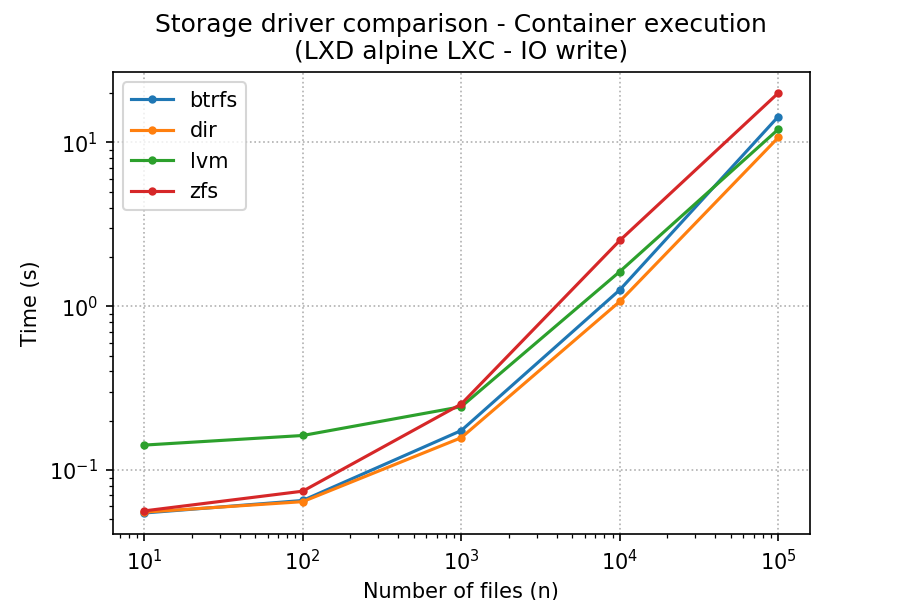
\includegraphics[width=\linewidth]{images/storage-driver/storage-driver-execution-LXD-alpine-LXC---IO-write.png}
      \caption{Average extracting time of n files from one (non-compressed) archive.}
      \label{fig:storage-driver:lxc:io-write-exec}
    \end{subfigure}
    
    \begin{subfigure}{.5\textwidth}
      \centering
      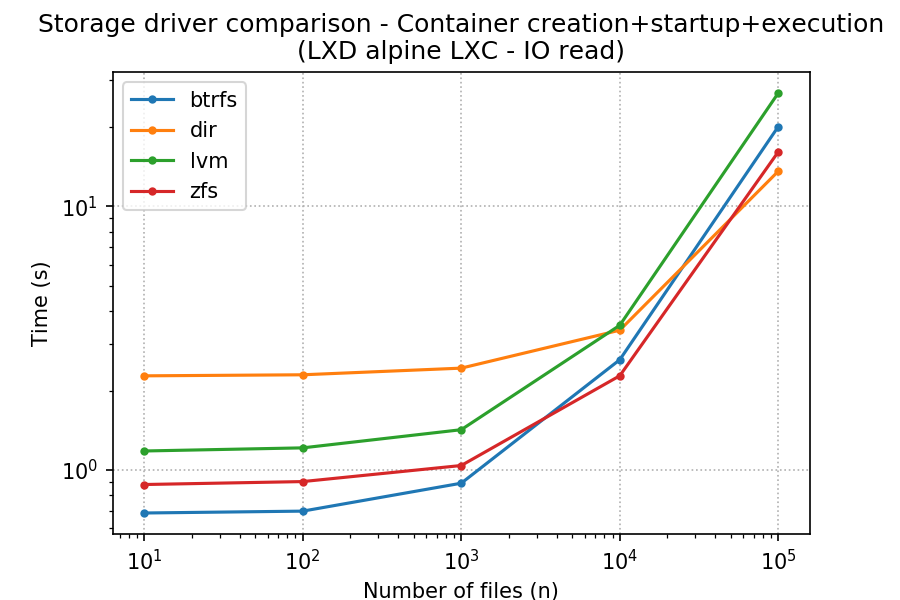
\includegraphics[width=\linewidth]{images/storage-driver/storage-driver-full-LXD-alpine-LXC---IO-read.png}
      \caption{Average creation, startup and execution time of containers used for IO reading performance test.}
      \label{fig:storage-driver:lxc:io-read-full}
    \end{subfigure}
    \begin{subfigure}{.5\textwidth}
      \centering
      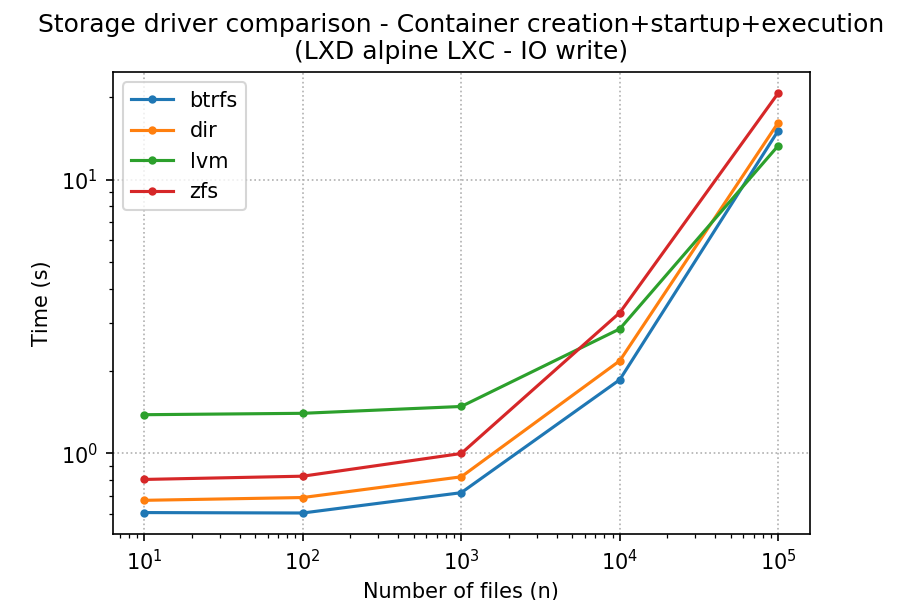
\includegraphics[width=\linewidth]{images/storage-driver/storage-driver-full-LXD-alpine-LXC---IO-write.png}
      \caption{Average creation, startup and execution time of containers used for IO reading performance test.}
      \label{fig:storage-driver:lxc:io-write-full}
    \end{subfigure}
    
    \caption{IO read and write tests for containers launched with Docker and runc, based on an Alpine image}
    \label{fig:storage-driver:lxc:io}
\end{figure}

LXD doesn't propose any file-based copy-on-write solution here.  We have dir, which corresponds to vfs for Docker, its full copy on creation is quite obvious on Figure \ref{fig:storage-driver:lxc:io-write-create}.  On Figure \ref{fig:storage-driver:lxc:io-read-create} though, it seems that all different storage driver suffer from the high amount of files to handle (still less than dir of course).  Overall, from Figure \ref{fig:storage-driver:lxc:db} and \ref{fig:storage-driver:lxc:io}, we can see that btrfs is the driver to go with, even though zfs provide decent execution performance, the cost of creating a container with that file system makes it not worth it to use it (for those tests at least).

\subsection{Container runtime}
The difference of implementation of the container runtime and the different isolation provided will mainly influence the time to execute different commands to interact with the container (like start and exec).  To illustrate that we will focus on the results obtained by different runtimes for the Hello World test.  We will only compare runc, crun, kata-runtime (qemu hypervisor) and kata-fc (firecracker hypervisor).  The common configuration will be:

\begin{tabular}{rl}
   \textbf{Container manager} & Docker \\
   \textbf{Container runtime} & overlay/devicemapper \\
   \textbf{Base image} & Alpine \\
   \textbf{Control group} & v1 \\
   \textbf{Rootless} & No 
\end{tabular}

The reason why we use both overlay and devicemapper in our tests is that overlay provide the best overal esperience, and ideally should be used, but as firecracker only support devicemapper, and given the considerable creation time overhead that this one has, it wouldn't be faire to compare it directly to the other runtime making use of overlay.

\begin{figure}[h!]
  \begin{center}
    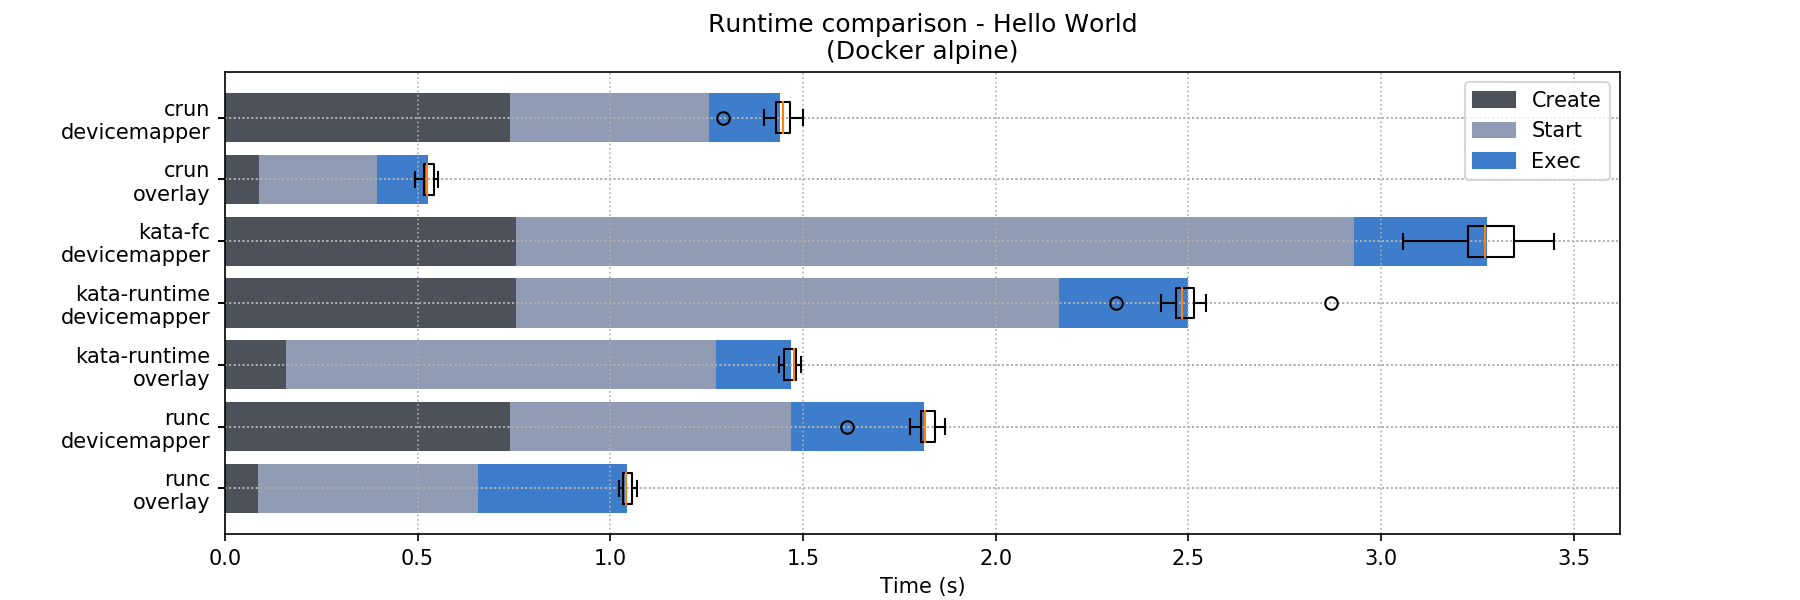
\includegraphics[width=\linewidth]{images/runtime/runtime-Hello-World-Docker-alpine.png}
    \caption{Hello World container test for different configurations}
    \label{fig:runtime:hello-world}
  \end{center}
\end{figure}

\begin{figure}[h!]

  \begin{subfigure}{.5\textwidth}
    \centering
    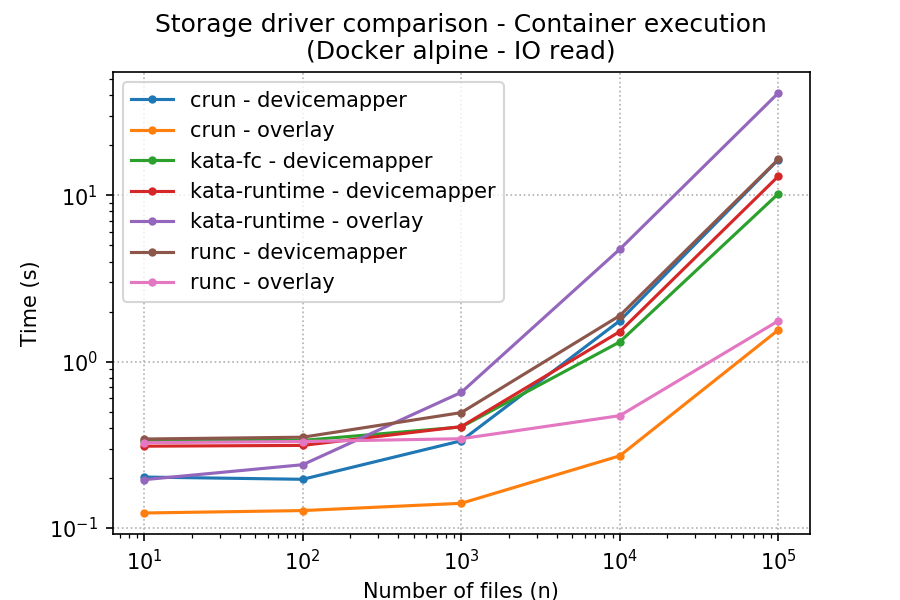
\includegraphics[width=\linewidth]{images/runtime/runtime-execution-Docker-alpine---IO-read.png}
    \caption{Average total reading time for n files.}
    \label{fig:runtime:io-read-exec}
  \end{subfigure}
  \begin{subfigure}{.5\textwidth}
    \centering
    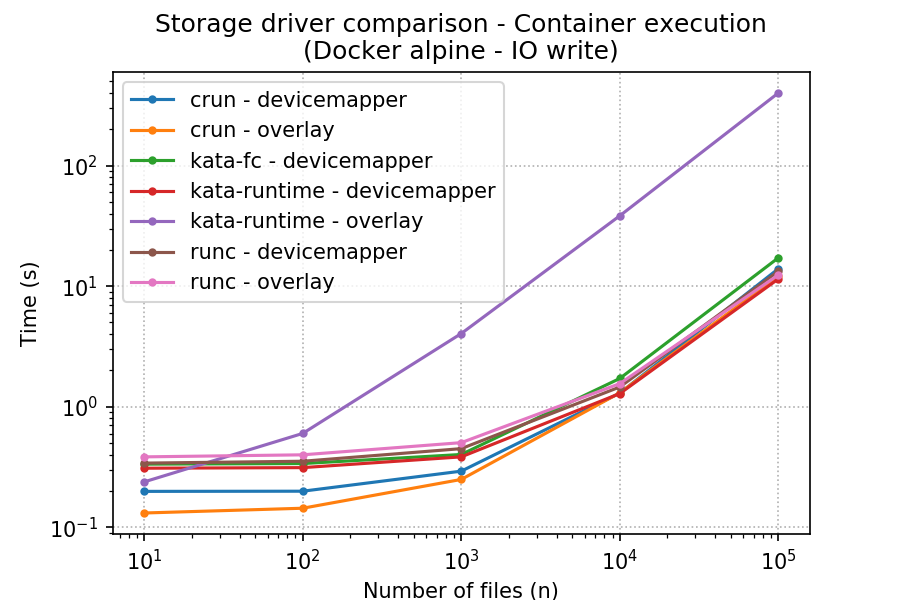
\includegraphics[width=\linewidth]{images/runtime/runtime-execution-Docker-alpine---IO-write.png}
    \caption{Average extracting time of n files from one (non-compressed) archive.}
    \label{fig:runtime:io-write-exec}
  \end{subfigure}
  
  \caption{}
  \label{fig:runtime:io}

\end{figure}

\begin{figure}[h!]
  
  \begin{subfigure}{.5\textwidth}
    \centering
    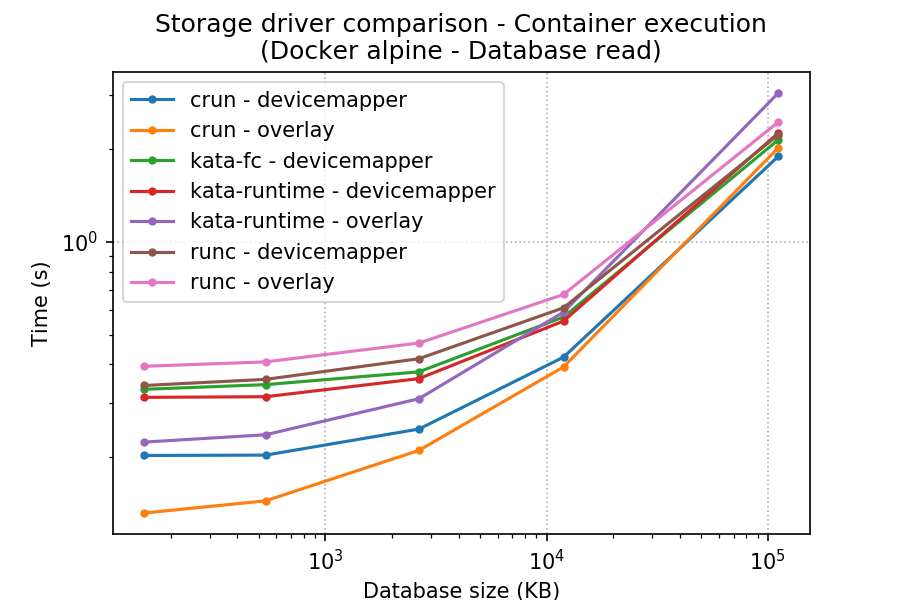
\includegraphics[width=\linewidth]{images/runtime/runtime-execution-Docker-alpine---Database-read.png}
    \caption{Average total reading time for n files.}
    \label{fig:runtime:db-read-exec}
  \end{subfigure}
  \begin{subfigure}{.5\textwidth}
    \centering
    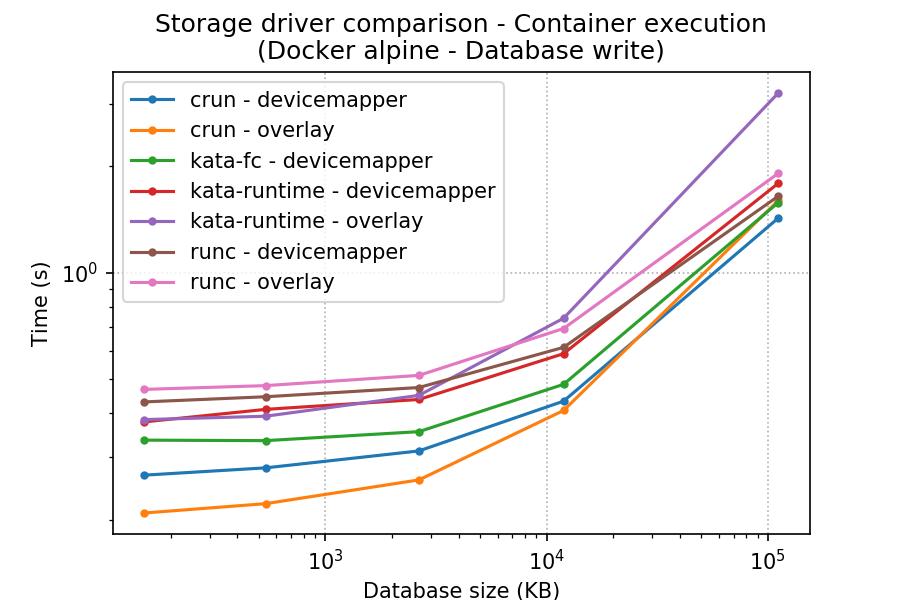
\includegraphics[width=\linewidth]{images/runtime/runtime-execution-Docker-alpine---Database-write.png}
    \caption{Average extracting time of n files from one (non-compressed) archive.}
    \label{fig:runtime:db-write-exec}
  \end{subfigure}
    
    \caption{}
    \label{fig:runtime:db}

\end{figure}

As expected, we can see on Figure \ref{fig:runtime:hello-world} that crun (implemented in c) is more efficient than runc (implemented in go).  We can also see that even though kata-runtime provide a stronger isolation using virutalization, its performances are not that far behind runc.  Kata-fc has a harder time keeping up though.  We can also see on Figure \ref{fig:runtime:io} and Figure \ref{fig:runtime:db} that crun keeps its advantage in execution time for I/O intensive tasks.

\clearpage
\subsection{Base image}
\begin{figure}[h!]
    \begin{subfigure}{.5\textwidth}
      \centering
      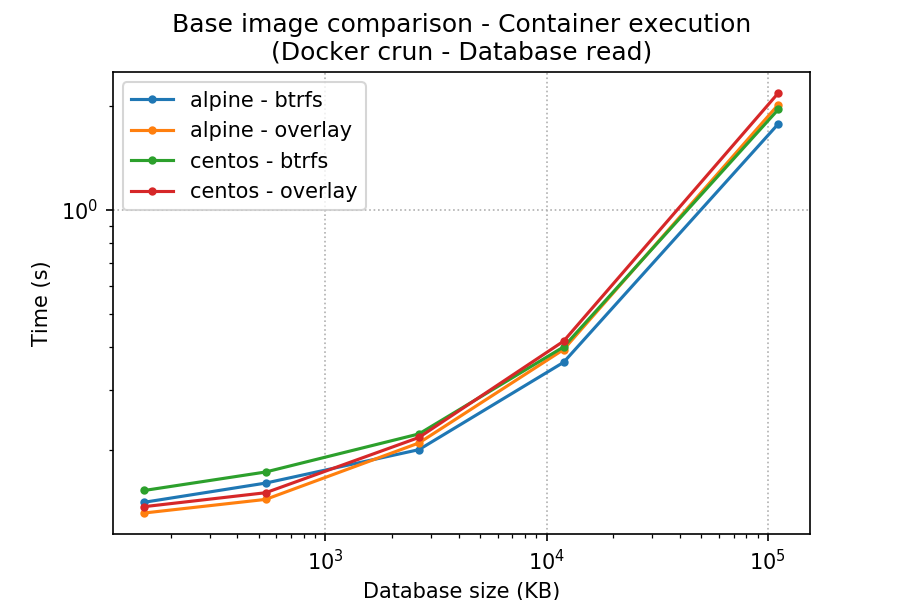
\includegraphics[width=\linewidth]{images/image/image-execution-Docker-crun---Database-read.png}
      \caption{Execution time of containers used for database reading performance test.}
      \label{fig:image:db-read-exec}
    \end{subfigure}
    \begin{subfigure}{.5\textwidth}
      \centering
      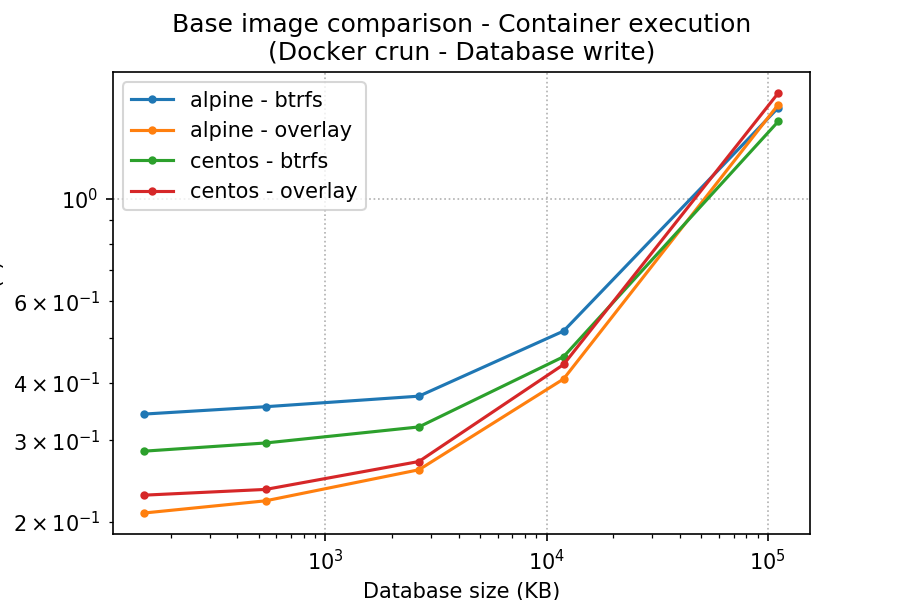
\includegraphics[width=\linewidth]{images/image/image-execution-Docker-crun---Database-write.png}
      \caption{Execution time of containers used for database reading performance test.}
      \label{fig:image:db-write-exec}
    \end{subfigure}
    
    \begin{subfigure}{.5\textwidth}
      \centering
      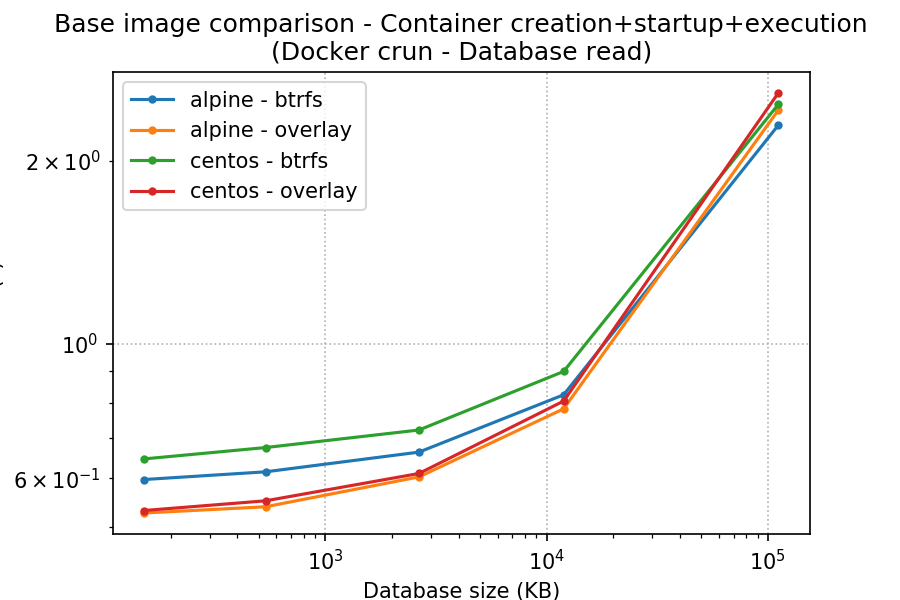
\includegraphics[width=\linewidth]{images/image/image-full-Docker-crun---Database-read.png}
      \caption{Creation, startup and execution time of containers used for database reading performance test.}
      \label{fig:image:db-read-full}
    \end{subfigure}
    \begin{subfigure}{.5\textwidth}
      \centering
      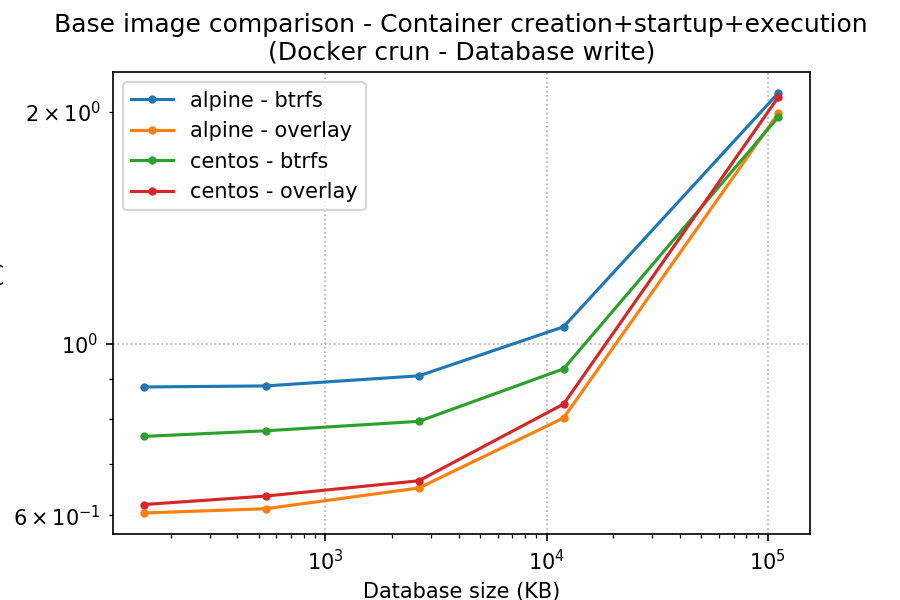
\includegraphics[width=\linewidth]{images/image/image-full-Docker-crun---Database-write.png}
      \caption{Creation, startup and execution time of containers used for database writing performance test.}
      \label{fig:image:db-write-full}
    \end{subfigure}
    
    \caption{Database read and write tests for containers launched with Docker and crun}
\end{figure}

\begin{figure}[!h]
    \begin{subfigure}{.5\textwidth}
      \centering
      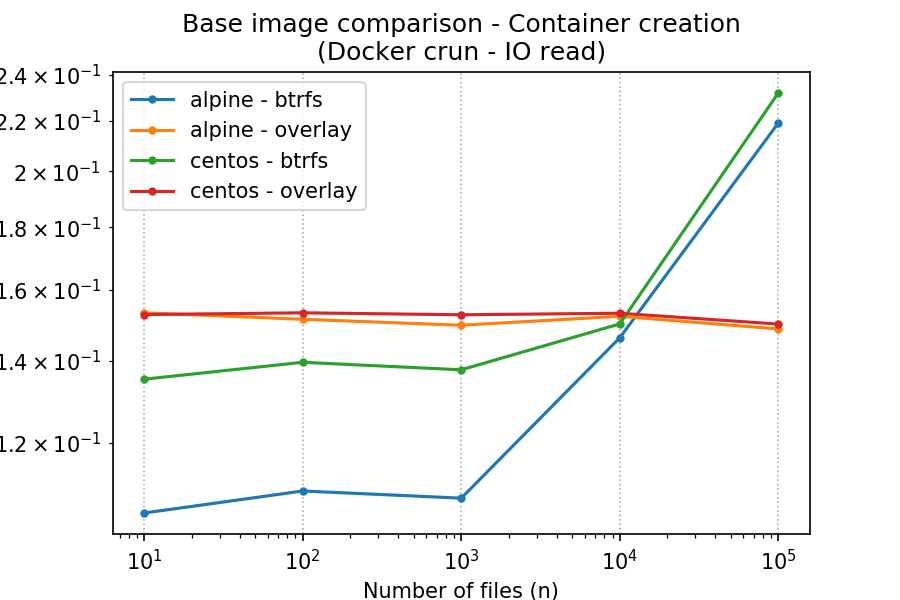
\includegraphics[width=\linewidth]{images/image/image-creation-Docker-crun---IO-read.png}
      \caption{Average creation time of containers depending on the number of files in one folder.}
      \label{fig:image:io-read-create}
    \end{subfigure}
    \begin{subfigure}{.5\textwidth}
      \centering
      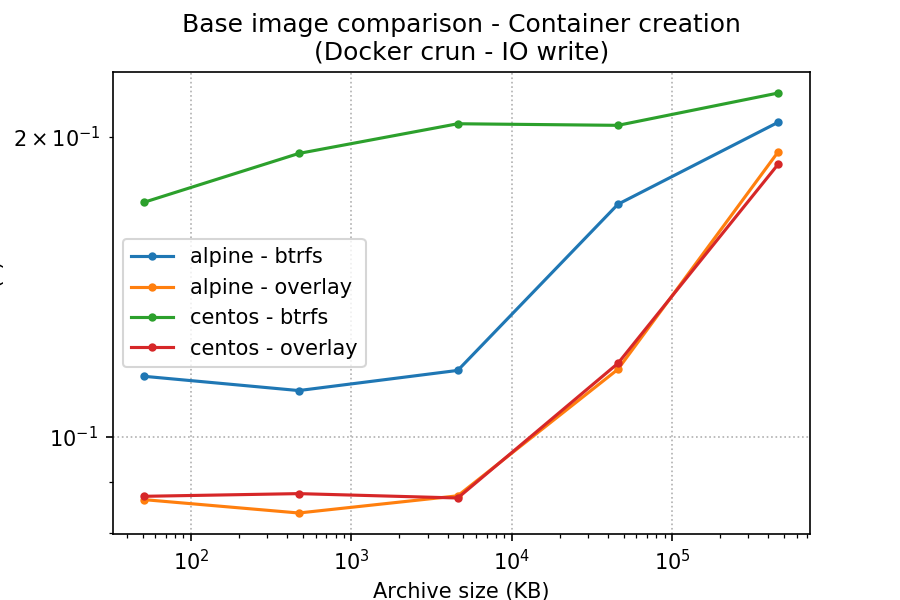
\includegraphics[width=\linewidth]{images/image/image-creation-Docker-crun---IO-write.png}
      \caption{Average creation time of containers depending on the size of the archive containing all the files.}
      \label{fig:image:io-write-create}
    \end{subfigure}
    
    % \begin{subfigure}{.5\textwidth}
    %   \centering
    %   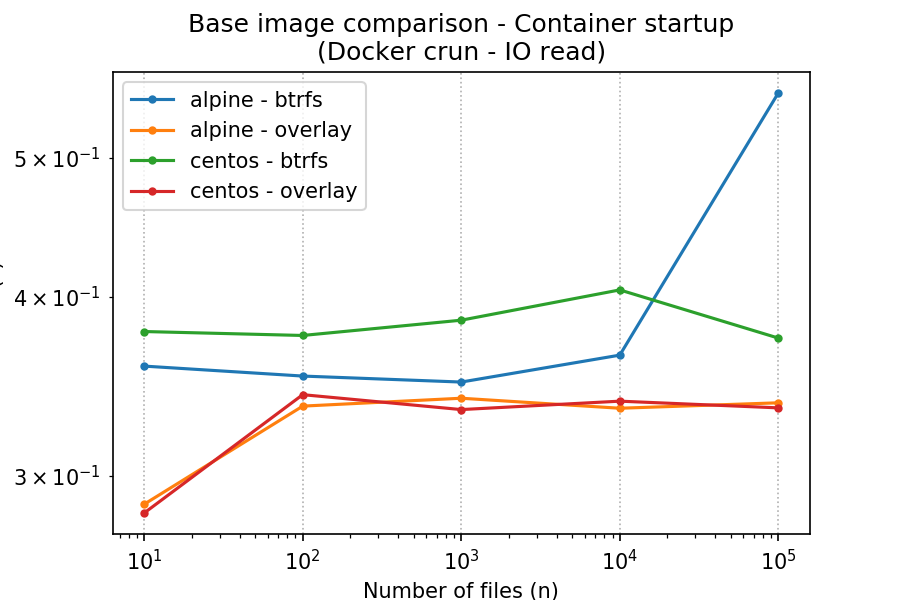
\includegraphics[width=\linewidth]{images/image/image-startup-Docker-crun---IO-read.png}
    %   \caption{Starting time of containers used for IO reading performance test.}
    %   \label{fig:image:io-read-start}
    % \end{subfigure}
    % \begin{subfigure}{.5\textwidth}
    %   \centering
    %   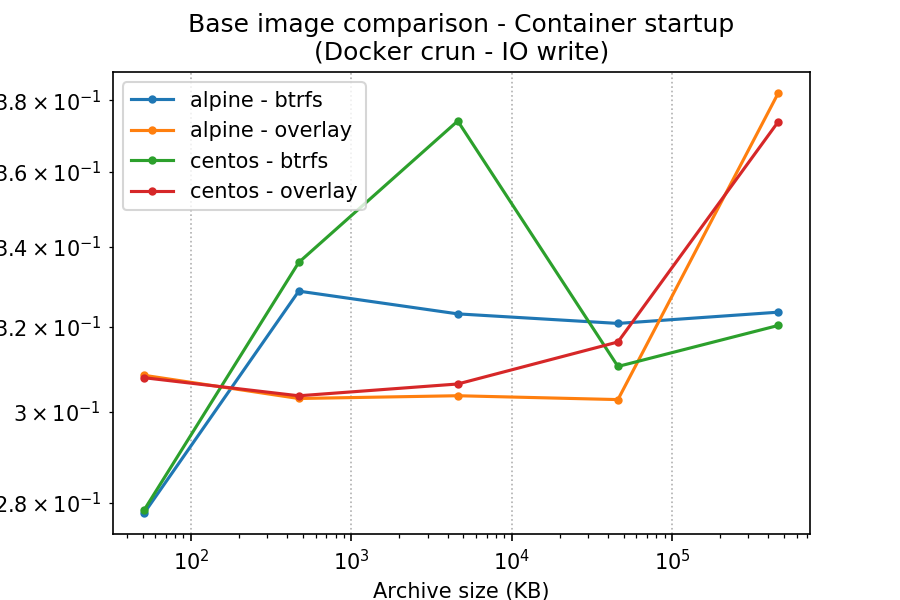
\includegraphics[width=\linewidth]{images/image/image-startup-Docker-crun---IO-write.png}
    %   \caption{Starting time of containers used for IO writing performance test.}
    %   \label{fig:image:io-write-start}
    % \end{subfigure}
    
    \begin{subfigure}{.5\textwidth}
      \centering
      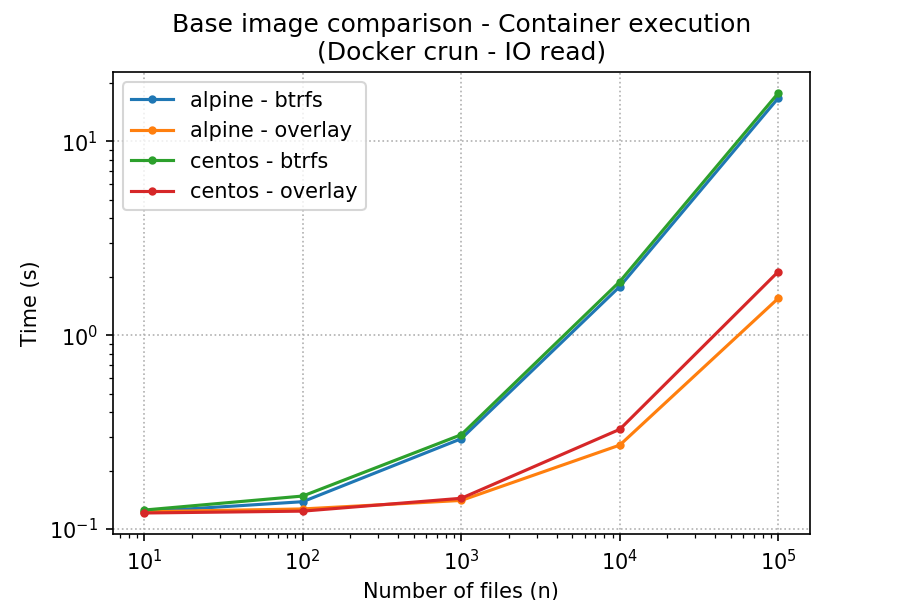
\includegraphics[width=\linewidth]{images/image/image-execution-Docker-crun---IO-read.png}
      \caption{Average total reading time for n files.}
      \label{fig:image:io-read-exec}
    \end{subfigure}
    \begin{subfigure}{.5\textwidth}
      \centering
      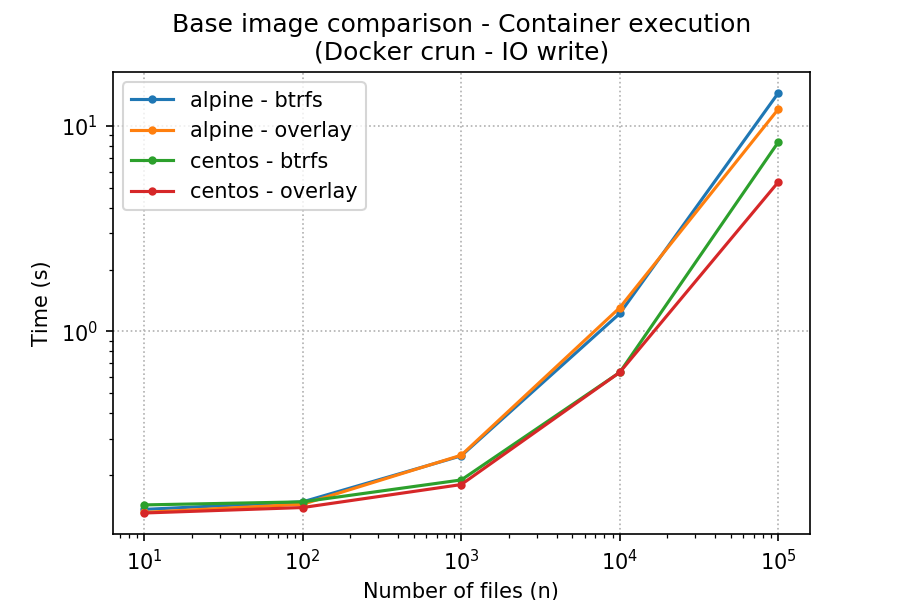
\includegraphics[width=\linewidth]{images/image/image-execution-Docker-crun---IO-write.png}
      \caption{Average extracting time of n files from one (non-compressed) archive.}
      \label{fig:image:io-write-exec}
    \end{subfigure}
    
    \begin{subfigure}{.5\textwidth}
      \centering
      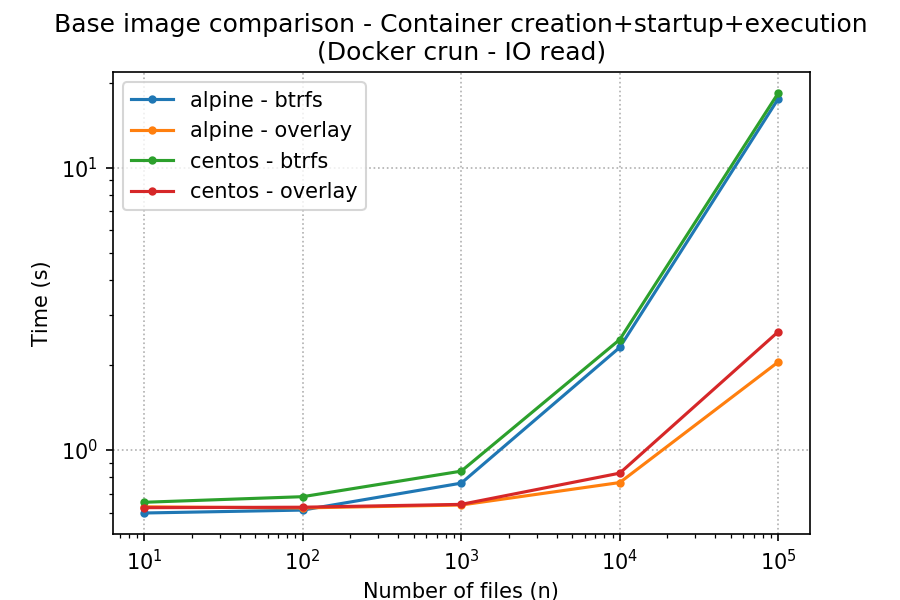
\includegraphics[width=\linewidth]{images/image/image-full-Docker-crun---IO-read.png}
      \caption{Average creation, startup and execution time of containers used for IO reading performance test.}
      \label{fig:image:io-read-full}
    \end{subfigure}
    \begin{subfigure}{.5\textwidth}
      \centering
      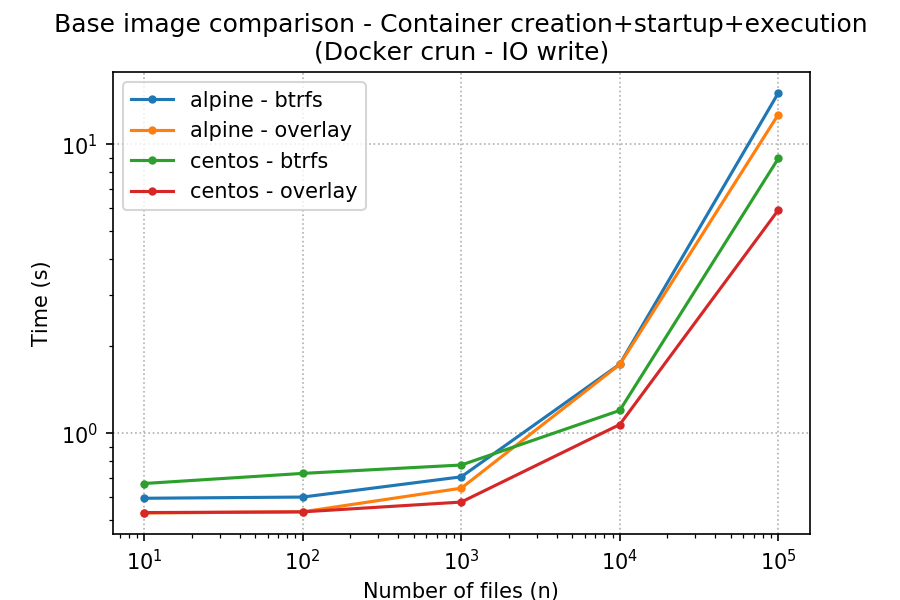
\includegraphics[width=\linewidth]{images/image/image-full-Docker-crun---IO-write.png}
      \caption{Average creation, startup and execution time of containers used for IO reading performance test.}
      \label{fig:image:io-write-full}
    \end{subfigure}
    
    \caption{IO read and write tests for containers launched with Docker and crun}
\end{figure}

\clearpage
\subsection{Rootless container}

\begin{figure}[h!]
  \begin{center}
    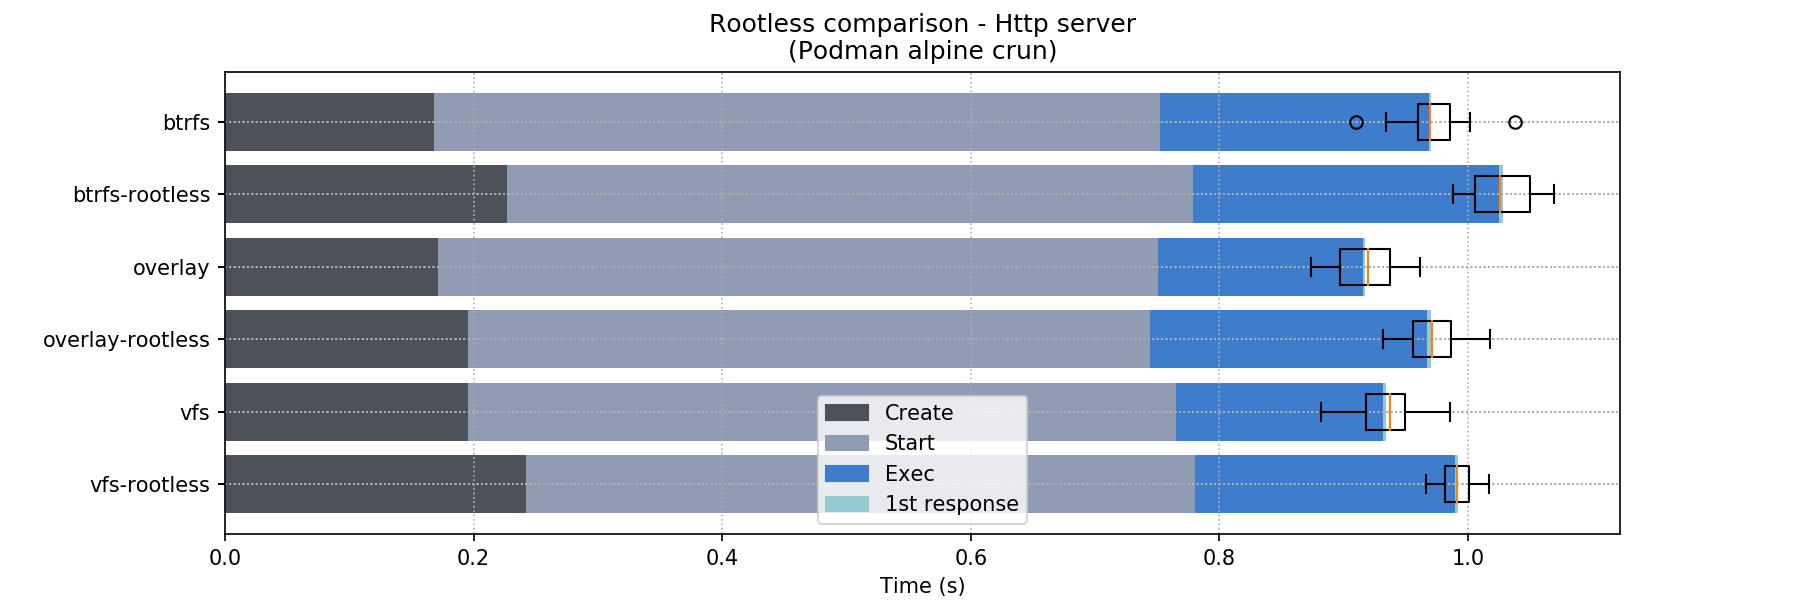
\includegraphics[width=\linewidth]{images/rootless/rootless-Http-server-Podman-alpine-crun.png}
    \caption{Hello World container test for different configurations}
    \label{fig:rootless:hello-world}
  \end{center}
\end{figure}

\begin{figure}[h!]
    \begin{subfigure}{.5\textwidth}
      \centering
      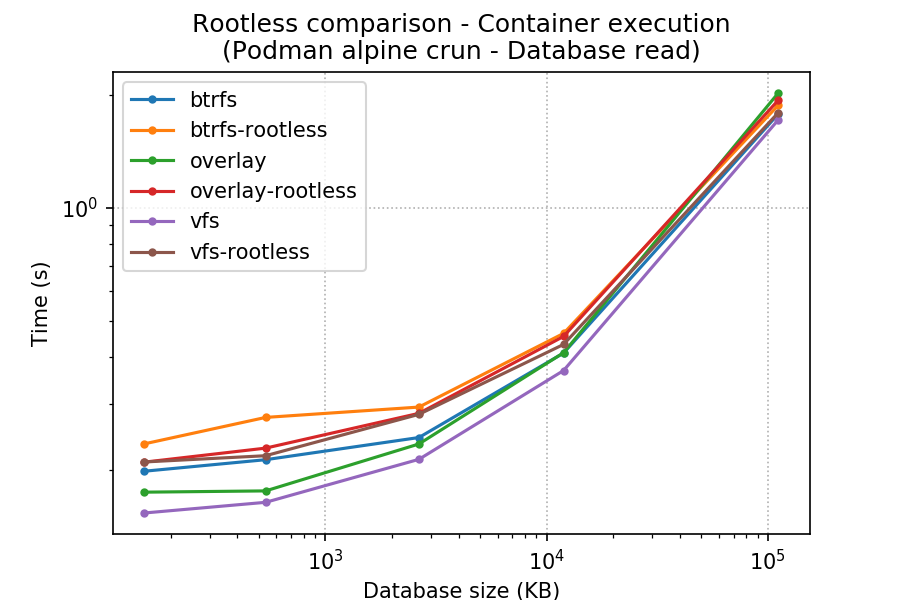
\includegraphics[width=\linewidth]{images/rootless/rootless-execution-Podman-alpine-crun---Database-read.png}
      \caption{Execution time of containers used for database reading performance test.}
      \label{fig:rootless:db-read-exec}
    \end{subfigure}
    \begin{subfigure}{.5\textwidth}
      \centering
      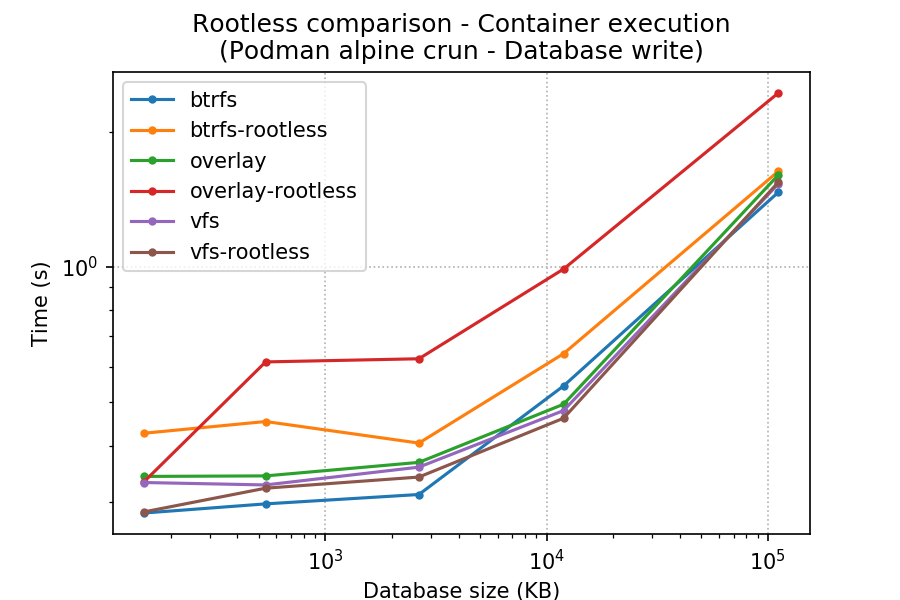
\includegraphics[width=\linewidth]{images/rootless/rootless-execution-Podman-alpine-crun---Database-write.png}
      \caption{Execution time of containers used for database reading performance test.}
      \label{fig:rootless:db-write-exec}
    \end{subfigure}
    
    \begin{subfigure}{.5\textwidth}
      \centering
      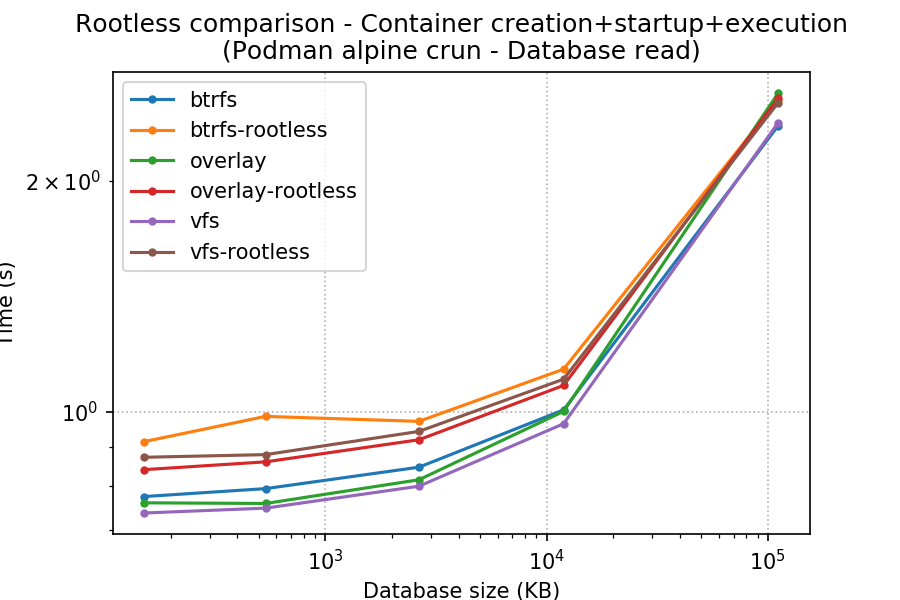
\includegraphics[width=\linewidth]{images/rootless/rootless-full-Podman-alpine-crun---Database-read.png}
      \caption{Creation, startup and execution time of containers used for database reading performance test.}
      \label{fig:rootless:db-read-full}
    \end{subfigure}
    \begin{subfigure}{.5\textwidth}
      \centering
      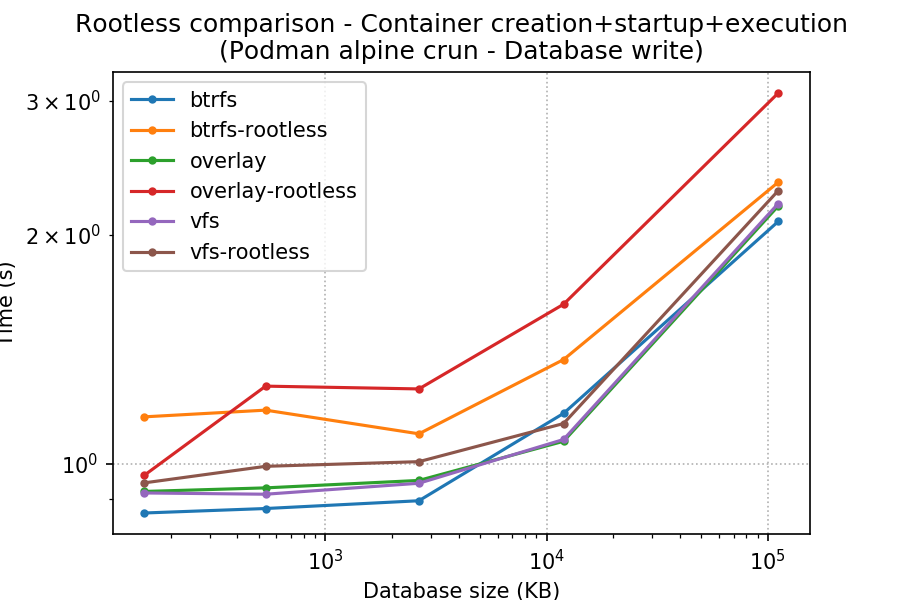
\includegraphics[width=\linewidth]{images/rootless/rootless-full-Podman-alpine-crun---Database-write.png}
      \caption{Creation, startup and execution time of containers used for database writing performance test.}
      \label{fig:rootless:db-write-full}
    \end{subfigure}
    
    \caption{Database read and write tests for containers launched with Podman and crun, based on an Alpine image}
    \label{fig:rootless:db}
\end{figure}

\begin{figure}[h!]
    \begin{subfigure}{.5\textwidth}
      \centering
      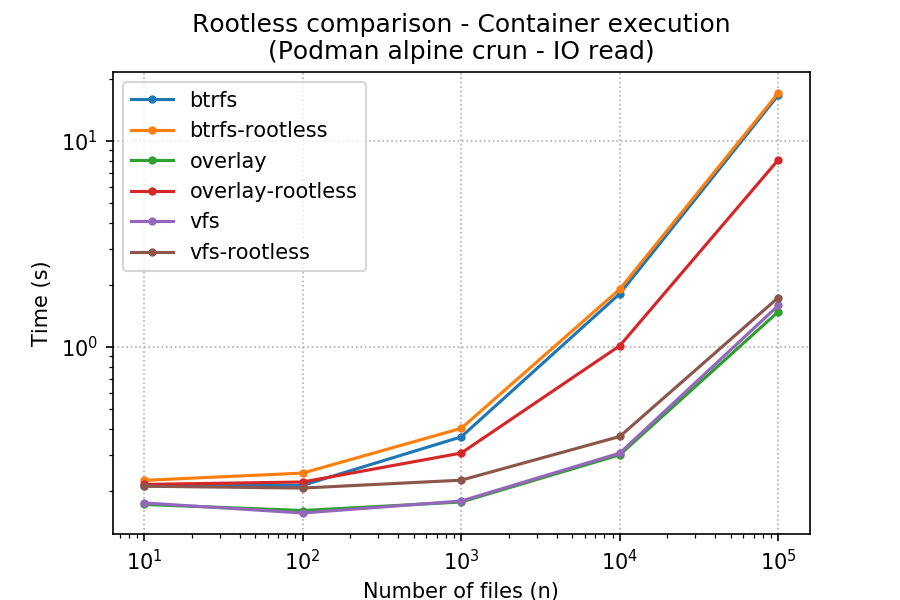
\includegraphics[width=\linewidth]{images/rootless/rootless-execution-Podman-alpine-crun---IO-read.png}
      \caption{Average total reading time for n files.}
      \label{fig:rootless:io-read-exec}
    \end{subfigure}
    \begin{subfigure}{.5\textwidth}
      \centering
      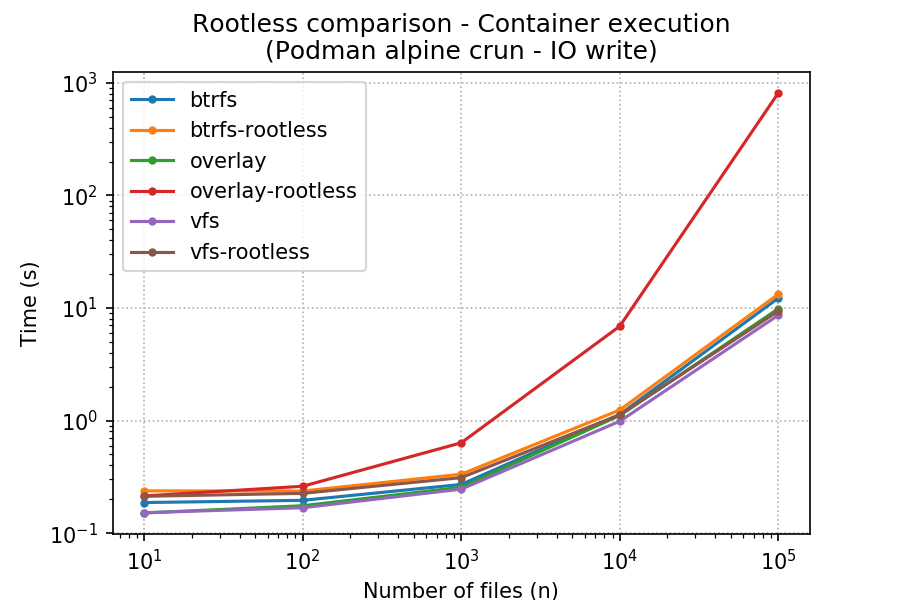
\includegraphics[width=\linewidth]{images/rootless/rootless-execution-Podman-alpine-crun---IO-write.png}
      \caption{Average extracting time of n files from one (non-compressed) archive.}
      \label{fig:rootless:io-write-exec}
    \end{subfigure}
    
    \begin{subfigure}{.5\textwidth}
      \centering
      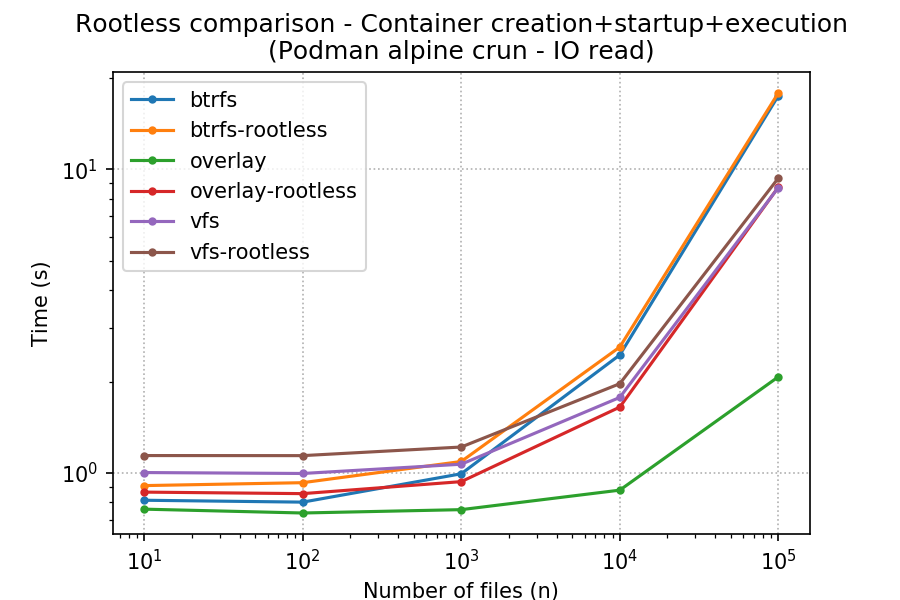
\includegraphics[width=\linewidth]{images/rootless/rootless-full-Podman-alpine-crun---IO-read.png}
      \caption{Creation, startup and execution time of containers used for IO reading performance test.}
      \label{fig:rootless:io-read-full}
    \end{subfigure}
    \begin{subfigure}{.5\textwidth}
      \centering
      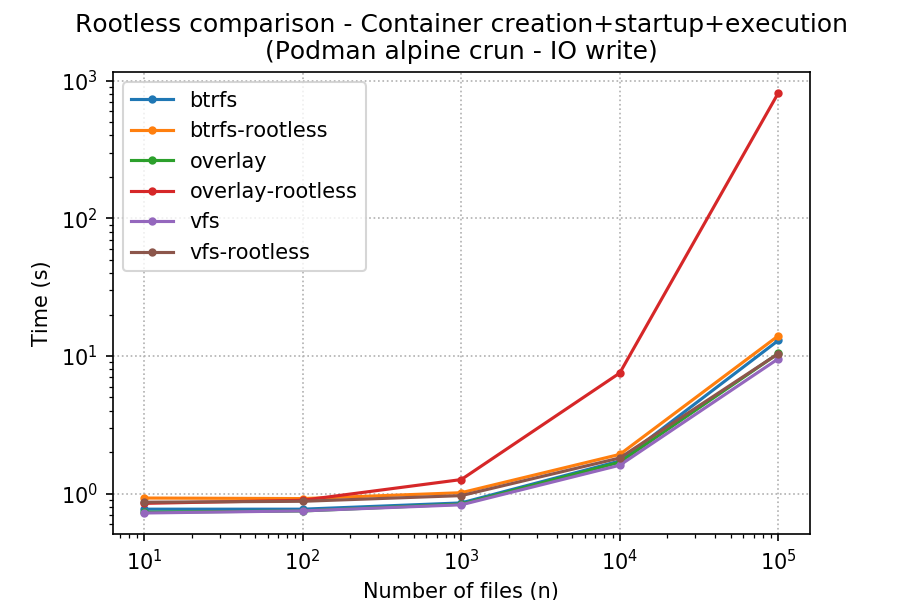
\includegraphics[width=\linewidth]{images/rootless/rootless-full-Podman-alpine-crun---IO-write.png}
      \caption{Creation, startup and execution time of containers used for IO writing performance test.}
      \label{fig:rootless:io-write-full}
    \end{subfigure}
    
    \caption{IO read and write tests for containers based on an Alpine image, launched with Podman and crun}
    \label{fig:rootless:db}
\end{figure}

\clearpage
\subsection{Container manager}

\begin{figure}[h!]
  \begin{center}
    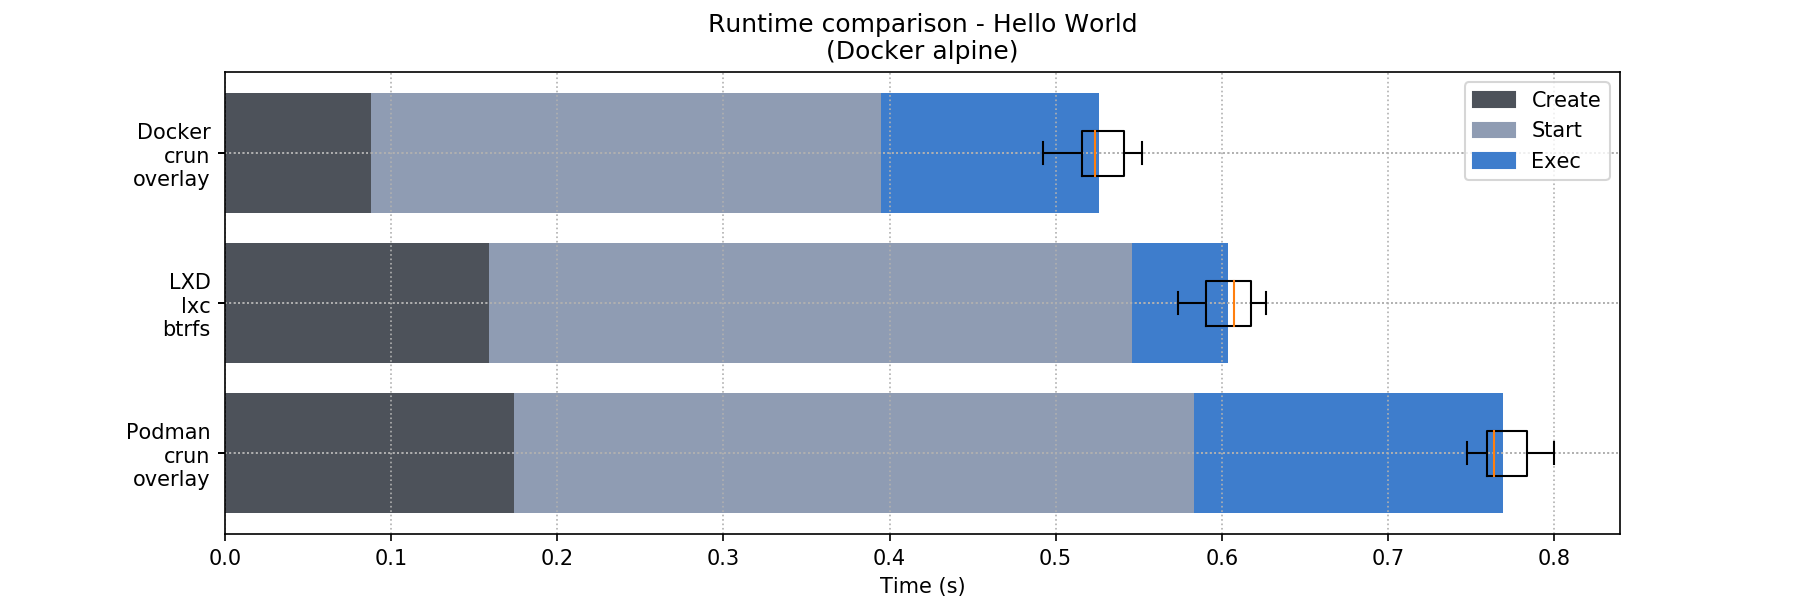
\includegraphics[width=\linewidth]{images/manager/manager-Hello-World-alpine.png}
    \caption{Hello World container test for different configurations}
    \label{fig:manager:hello-world}
  \end{center}
\end{figure}

\begin{figure}[h!]
    \begin{subfigure}{.5\textwidth}
      \centering
      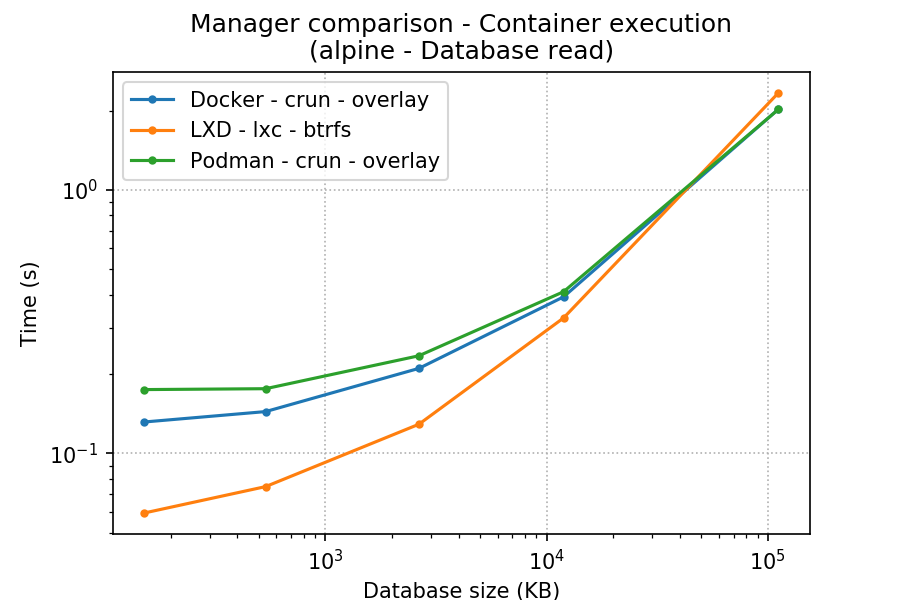
\includegraphics[width=\linewidth]{images/manager/manager-execution-alpine---Database-read.png}
      \caption{Execution time of containers used for database reading performance test.}
      \label{fig:manager:db-read-exec}
    \end{subfigure}
    \begin{subfigure}{.5\textwidth}
      \centering
      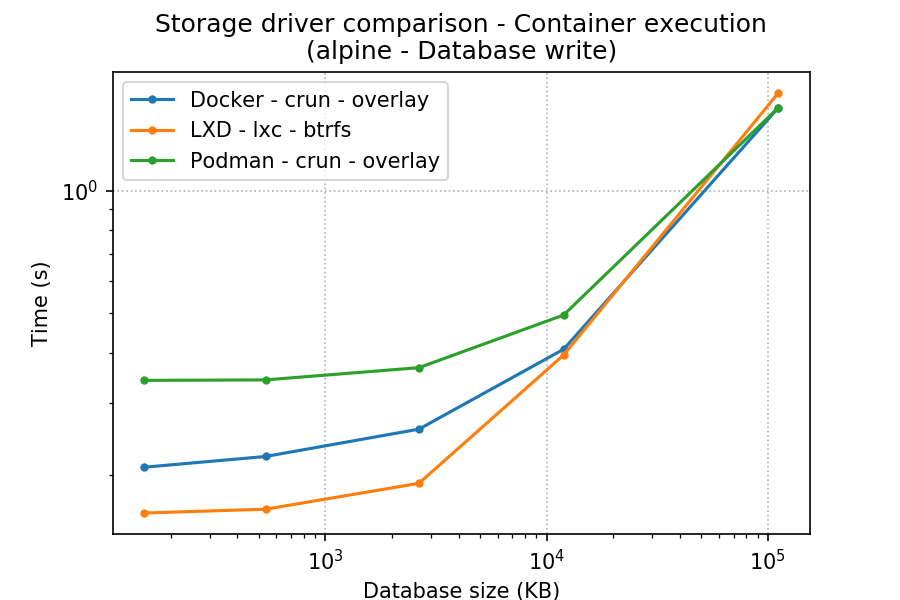
\includegraphics[width=\linewidth]{images/manager/manager-execution-alpine---Database-write.png}
      \caption{Execution time of containers used for database reading performance test.}
      \label{fig:manager:db-write-exec}
    \end{subfigure}
    
    \begin{subfigure}{.5\textwidth}
      \centering
      \includegraphics[width=\linewidth]{images/manager/manager-full-alpine---Database-read.png}
      \caption{Creation, startup and execution time of containers used for database reading performance test.}
      \label{fig:manager:db-read-full}
    \end{subfigure}
    \begin{subfigure}{.5\textwidth}
      \centering
      \includegraphics[width=\linewidth]{images/manager/manager-full-alpine---Database-write.png}
      \caption{Creation, startup and execution time of containers used for database writing performance test.}
      \label{fig:manager:db-write-full}
    \end{subfigure}
    
    \caption{Database read and write tests for containers based on an Alpine image}
    \label{fig:manager:db}
\end{figure}

\begin{figure}[h!]
    \begin{subfigure}{.5\textwidth}
      \centering
      \includegraphics[width=\linewidth]{images/manager/manager-execution-alpine---IO-read.png}
      \caption{Average total reading time for n files.}
      \label{fig:manager:io-read-exec}
    \end{subfigure}
    \begin{subfigure}{.5\textwidth}
      \centering
      \includegraphics[width=\linewidth]{images/manager/manager-execution-alpine---IO-write.png}
      \caption{Average extracting time of n files from one (non-compressed) archive.}
      \label{fig:manager:io-write-exec}
    \end{subfigure}
    
    \begin{subfigure}{.5\textwidth}
      \centering
      \includegraphics[width=\linewidth]{images/manager/manager-full-alpine---IO-read.png}
      \caption{Creation, startup and execution time of containers used for IO reading performance test.}
      \label{fig:manager:io-read-full}
    \end{subfigure}
    \begin{subfigure}{.5\textwidth}
      \centering
      \includegraphics[width=\linewidth]{images/manager/manager-full-alpine---IO-write.png}
      \caption{Creation, startup and execution time of containers used for IO writing performance test.}
      \label{fig:manager:io-write-full}
    \end{subfigure}
    
    \caption{IO read and write tests for containers based on an Alpine image}
    \label{fig:manager:db}
\end{figure}

\clearpage
\section{Best overal solution}
